\chapter{Konzolová časť aplikácie na správu mikrotikov}
V tejto kapitole sa popisuje fungovanie naprogramovanej aplikácie. Celkovo je konzolová časť aplikácie napísaná za pomoci knižnice tikapy popísanej v kapitole \ref{sec:tikapy}. Kapitola bude rozdelená do niekoľkých častí:\begin{itemize}
\item Časť 1: popis naprogramovanej časti pre vyhľadávanie mikrotikov, pripojenie sa na mikrotik cez python pomocou protokolov telnet, SSH, mactelnet a napojenie na metódy
\item Časť 2: Popis infraštruktúry backendu - zložky, ich vysvetlenie, zoznam súborov na konfiguráciu mikrotku, vysvetenie rozdelenia, vysvetlenie tried, metód daných tried a volanie funkcií
\item časť 3 - pridanie tabuliek jednotlivých tried a ich metód v každej zložke, krátka sumarizácia, ich niektoré vybrané UML diagramy
\end{itemize}
\section{Popis naprogramovanej časti prihlasovania na mikrotik}
\label{sec:popis1}
V tejto časti sa zobrazí rozbor časti prihlasovania na mikrotik a jeho základné funnkcie. Toto je riadené v rámci projektu nazvaného \textit{diplomkap3} v ktorom je súbor \textit{loginManager.py}. V rámci login managera tu nachádzame ďalšie súbory, ktoré sú zobrazené na obrázku \ref{fig:filesLogin}. 
\begin{figure}[H]
\centering
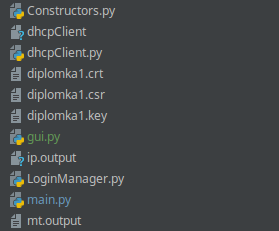
\includegraphics[scale=0.6]{../text/loginFiles.png}
\caption{Zoznam základných konfiguračných súborov}
\label{fig:filesLogin}
\end{figure} 
\subsection{Súbor centralControl}
\label{sec:central}
V súbore centrolControl sa popisuje spôsob hromadnej obsluhy mikrotikov na základe protokolu mactelnet. Pozostáva z metód:
\begin{itemize}
\item \textit{konštruktor} - Pozostáva z užívateľských mien a hesiel, heslá v premennej credentials sú uložené ako slovník v podobe IP adresa: heslo
\item \textit{listMikrotikDevices()} - metóda vráti zoznam MAC a IP adries nájdených mikrotikov, uloží ich do súboru, a finálny výstup predstavuje list MAC adries
\item \textit{addCredentials()} - metóda pridáva heslo k užívateľskému účtu do slovníku, štandardné užívateľské meno sa používa admin, ale tiež sa môže použiť aj iné užívateľské meno pri volaní metódy
\item \textit{loginSSH()}- metóda je použitá na hromadné prihlásenie pomocou protokolu SSH na mikrotiky, používa sa tu pritom knižnica pexpect a jej subkižnica pxssh, jej vstupné parametre sú IP adresa serveru, užívateľské meno a heslo 
\end{itemize}
\linebreak
\begin{lstlisting}[language=python, frame=single, caption=Deklarácia vstupných parametrov,captionpos=b]
 def __init__(self, login):
        self.username = login
        self.credentials = {
            "192.168.1.1": "admin",
            "192.168.2.1": ""
\end{lstlisting}
\begin{lstlisting}[language=python, frame=single, caption=Meóda zobrazenia mikrotikov,captionpos=b, showstringspaces=false]
 def listMikrotikDevices(self):
   deviceList = []
   loadAddress = False
   os.system("mactelnet -l -t 20 2>&1 > mt.output")
    with open( "mt.output", "r" ) as file:
     for line in file:
      if loadAddress:
         address = line.split( )[0]
         deviceList.append( address )
      else:
         header = line.split( )
         if len( header ) > 1:
            if "IP" in header[0]:
              loadAddress = True
  return deviceList
\end{lstlisting}
\newpage
\begin{lstlisting}[language=python, frame=single, caption=Metóda pridania užívateľských mien a hesiel,captionpos=b, showstringspaces=false]
 def addCredentials(self, login="admin"):
   server_list = self.listMikrotikDevices()
   print( server_list )
   for server in server_list:
   try:
    password = self.credentials[server]
    except KeyError:
    password = input( "Please eneter the 
    password for " + server + ":" )
    self.credentials[server] = password
    return server_list
\end{lstlisting}
\begin{lstlisting}[language=python, frame=single, caption=Metóda hromadného prihlásenia pomocou protokolu SSH,captionpos=b, showstringspaces=false]
 def loginSSH(self, server,login, password):
 from pexpect import pxssh, spawn, expect
 import getpass
 for server in self.credentials:
 try:
  connect = pxssh.pxssh( )
  server = self.credentials
  login = 'admin'
  password = self.credentials[server]
  port = 22
  connect.login( server, login, password )
  commands = pxssh.spawn( )
  time.sleep( 10 )
 except pxssh.ExceptionPxssh as e:
  print( "Error" )
  print( str( e ) )
\end{lstlisting}
\subsection{Súbor Constructors}
Súbor predstavuje zoznam konštruktorov pre konkrétne naprogramované API moduly pomocou knižnice tikapy. V úvode konštruktoru sú popísané importy jednotlivých modulov a submodulov pre konfiguráciu mikrotiku za pomoci API. \\
Následne je vytvorená trieda Mikrotik, ktorá zahŕňa všetky konštruktory spoločne s ich vstupnými parametrami, ktoré sú adresa,užívateľské meno a heslo. 
\begin{figure}[H]
\centering
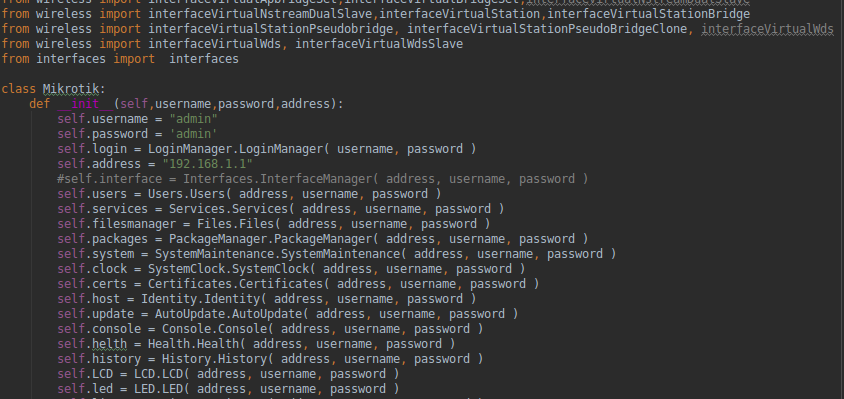
\includegraphics[scale=0.5]{../text/constructors.png}
\caption{Ukážka konštruktorov projektu}
\label{fig:constructors}
\end{figure} 
\subsection{Súbor dhcpClient}
V tomto súbore sa nachádza základná konfigurácia mikrotiku po pripojení naň. Obsahuje triedu basicConfig, ktorá pozostáva z dvoch metód.\\
V konštruktore sa nastaví rozhranie, na ktorom sa má adresa nastaviť, IP adresa/subnet a MAC adresa na pripojenie na mikrotik pomocu protokolu mactelnet.
\begin{lstlisting}[language=python, frame=single, caption=Trieda basicConfig,captionpos=b, showstringspaces=false]
 class basicCOnfig:
    def __init__(self,interface,mac,ip):
        self.interface = interface
        self.mac = mac
        self.ip = ip
\end{lstlisting}
Prvá metóda \textit{dhcp()}, ktorej vstupné parametre sú užívateľské meno a heslo. Pozostáva z prihlásenia na mikrotik, a nastavenia Dynamic Host Client Protocol (DHCP) klienta na rozhraní, ktoré sa definuje pri volaní objektu v rámci konštruktoru.
\newpage
\begin{lstlisting}[language=python, frame=single, caption=Metóda dhcp,captionpos=b, showstringspaces=false]
 def dhcp(self,username,password):
        child =pexpect.spawn('mactelnet '+self.mac)
        child.expect('Username:')
        child.sendline(username)
        child.expect('Password:')
        child.sendline(password)
        child.sendline('\r')
        try:
            child.expect('> ')
            child.sendline('ip dhcp-client add 
            interface='+self.interface+"\r")
            child.expect('> ')
            child.close()
        except:
            child.close()
\end{lstlisting}
Druhá metóda \textit{setAddress()}, ktorá bere ako vstupné parametre užívateľské meno a heslo nastaví statickú IP adresu na rozhraní definovanom v rámci konštruktoru.
\begin{lstlisting}[language=python, frame=single, caption=Metóda setAddress,captionpos=b, showstringspaces=false]
 def setAddress(self,username,password):
        child = pexpect.spawn( 'mactelnet '+ 
        self.mac )
        child.expect( 'Username:' )
        child.sendline( username )
        child.expect( 'Password:' )
        child.sendline( password )
        child.sendline( '\r' )
        try:
            child.expect( '> ' )
            child.sendline( 'ip address add address='+self.ip 
            +"interface="+self.interface+"\r" )
            child.expect( '> ' )
            child.close()
        except:
            child.close()
\end{lstlisting}
\subsection{Súbor LoginManager}
Súbor LoginManager pozostáva z niekoľkých metód, tieto metódy majú podobnú štruktúru ako súbor centralConrol popisujúci v kapitole \ref{sec:central}.\\
Ako prvá popísaná časť je konštruktor, ktorý prijíma vstupné parametre užívateľské meno a heslo.
\begin{lstlisting}[language=python, frame=single, caption=Konštruktor súboru,captionpos=b, showstringspaces=false] 
def __init__(self, login,password):
        self.username = login
        self.pwd = password
\end{lstlisting}
Druhá metóda je metóda \textit{loginTelnet()},v rámci tejto metódy sa rieši prihlásenie na mikrotik pomocou protokolu telnet za použitia knižnice telnetlib. Vo vstupe metódy sa definuje premenná \textit{server\_ list}. Táto premenná je naplnená IP adresami mikrotikov v rámci súboru centralControl.
\begin{lstlisting}[language=python, frame=single, caption=Metóda loginTelnet,captionpos=b, showstringspaces=false] 
def loginTelnet(self, password, login="admin"):
        import telnetlib
        central = centralControl(login, password)
        server_list = central.listMikrotikDevices()
        print(server_list)
        for server in server_list:
            try:
                telnetcon = telnetlib.Telnet
                ( host=server, port=23 )
                telnetcon.read_until( b"Login: " )
                telnetcon.write( login.encode( )
                 + "\n" )
                telnetcon.read_until( b"Password: " )
                telnetcon.write( password.encode( )
                 + b"\n" )
                time.sleep( 10 )
                telnetcon.close( )
            except:
                print( "Cannot connect to 
                router via telnet" )
\end{lstlisting}
\newpage
Ďalej sa tu nachádza metóda \textit{loginSSH()}, táto metóda pracujúca podobne ako metoda loginTelnet() pracuje na základe protokolu SSH, na vstupe má server IP adresu, užívateľské meno  a heslo.
\begin{lstlisting}[language=python, frame=single, caption=Metóda loginSSH,captionpos=b, showstringspaces=false] 
def loginSSH(self, server,login, password):
        from pexpect import pxssh, spawn, expect
        import getpass
        try:
            connect = pxssh.pxssh( )
            server = '172.16.49.2'
            login = 'admin'
            password = 'admin'
            port = 22
            connect.login( server, login, 
            password )
            commands = pxssh.spawn( )
            time.sleep( 10 )
        except pxssh.ExceptionPxssh as e:
            print( "Error" )
            print( str( e ) )
\end{lstlisting}
Ďalšou metódou je metóda na vylistovanie všetkých mikrotikov, táto metóda je bez vstupného parametru. Ako výstup je súbor \textit{mikrotik.output} naplnený MAC adresami mikrotikov. 
\newpage
\begin{lstlisting}[language=python, frame=single, caption=Metóda listMikrotikDevices,captionpos=b, showstringspaces=false] 
def listMikrotikDevices(self):
        deviceList = []
        loadMacAddress = False
        os.system("mactelnet -l -t 20 
        2>&1 > mt.output")
        with open( "mt.output", "r" ) 
        as file:
            for line in file:
                if loadMacAddress:
                   macAddress = line.split( )[1]
                   deviceList.append( macAddress )
                else:
                    header = line.split( )
                    if len( header ) > 1:
                        if "IP" in header[0] 
                        and "MAC-Address" 
                        in header[1]:
                            loadMacAddress = True
        return deviceList
\end{lstlisting}
Poslednou metódou je metóda \textit{mactelnetLoginToSingleDevice()}, vďaka ktorej sa pripája pomocou protokolu mactelnet na jedno mikrotik zariadenie pomocou MAC adresy získanej z výstupu metódy \textit{listMikrotikDevices()} mikrotik.output.
\newpage
\begin{lstlisting}[language=python, frame=single, caption=Metóda mactelnetLoginToSingleDevice,captionpos=b, showstringspaces=false] 
def mactelnetLoginToSingleDevice(self, username, 
    password, address=None):
        deviceList = self.listMikrotikDevices()
        print( deviceList )
        if address:
            print('mactelnet {} -u {} -p {}'.format
            ( address, username, password ))
            os.system( 'mactelnet {} -u {} -p {}'.format
            ( address, username, password ) )
        elif deviceList:
            print( 'mactelnet {} -u {} -p {}'.format
            ( deviceList[0], username, password ) )
            os.system( 'mactelnet {} -u {} -p {}'.format
            ( deviceList[0], username, password ) )
        else:
            print("No device was found")
\end{lstlisting}
\section{Rozbor hlavnej časti backendu}
V rámci hlavnej konfiguračnej časti diplomovej práce, pre konfiguráciu backendu mikrotiku za pomoci programovacieho jazyka python som projekt rozdelil do niekoľkých častí:\begin{itemize}
\item \textbf{bridge} - táto časť obsahuje prvky konfiguácie, pridania, odstránenia, zapnutia, vypnutia možnosti bridgu na mikrotiku, konfigurácia existujúceho bridgu, zobrazenie zoznamu bridgov
\item  \textbf{capsman} - Táto časť obsahuje konfiguráciu hromadnej obsluhy mikrotik prístupových bodov a WiFi, profily, bezpečnosť, konfiguácie, povolené rýchlosti, zobrazenie zoznamu pripojených prvkov a ďalšie funkcie
\item \textbf{certs} - Obsahuje certifikáty na pripojenie sa na mikrotik pomocou protokolu API-SSL
\item \textbf{Dude} - Obsahuje popis konfigurácie ako nastaviť nástroj Dude klienta, ako nakonfigurovať Dude na vzdialený monitoring na Dude serveri, taktiež Dude server, a ďalšie možnosti
\item \textbf{exportToHtml} - Časť predstavuje generovanie súboru na analýzu v podobe webovej stránky
\item \textbf{interfaces} - Časť predstavuje konfiguráciu rozhraní na mikrotiku, tieto časti sú tiež popísané aj v iných zložkách ako napr. bridge. časť popisuje pridanie, odstránenie, zapnutie, vypnutie, konfiguráciu existujúcich rozhraní.
\item \textbf{IPv4} - Rozsiahla časť, obsahuje konfiguráciu IP adries, firewallu, monitoringu, smerovania a ďalších nástrojov spadajúcich pod IP zložku na mikrotiku.
\item \textbf{IPv6} - Pre zložku IPv6 platí to isté čo pre zložku IPv4, ale platí pre konfiguráciu na základe IPv6 adresného rozsahu
\item \textbf{KVM} - Sekcia bude popisovať možnosti virtualizácie mikrotiku.
\item \textbf{log} - Sekcia bude popisovať analýzu a konfiguráciu logu zariadenia
\item \textbf{makeSupportFile} - Seckia bude popisovať vytvorenie súboru potrebného pre analýzu na mikrotik podpore
\item \textbf{mesh} - Sekcia popisuje konfiguráciu tzv. mesh technológie, technológii podobne ako  v rámci časti bridge
\item \textbf{MPLS} - Sekcia bude popisovať možnosti konfiurácie Multi Protocol Label Switching (MPLS), jej pridanie, odstránenie ,zapnutie, vypnutie, modifikácie a ďalšie funkcie.
\item \textbf{PPP} - sekcia bude popisovať konfiguráciu Point to Point Protocol (PPP) a ďalších možností Virtual Private Network (VPN) konfigurácie.
\item \textbf{Queues} - Sekcia budep popisovať konfiguráciu sieťových front, možnosti front, typy front a ďalšie funkcie
\item \textbf{Radius} - Sekcia bude popisovať nastavenie funkcie Radius - autentizačnej služby užívateľov , jeho modifikáciu, konfiguráciu a ďalšie funkcie.
\item \textbf{Routing} - Sekcia bude popisovať možnosti dynamického smerovania, statické smerovanie bude popísané v rámci časti IPv4, dynamické smerovacie protokoly, ich konfigurácie, a ďalšie možnosti. 
\item \textbf{Switch} - Sekcia bude popisovať konfiguráciu prepínača, niektoré mikrotiky sú typu SwitchOS a sú štandardne prepínač. Kofiguuráciu portov, trunkov, a ďalších funkcií. 
\item \textbf{System} - Sekcia bude popisovať časť konfigurácie systémových nástrojov, ich funkcií a konfigurácie, a ďalších funkcií.
\item \textbf{Tools} - Sekcia bude popisovať konfiguráciu mikrotik nástroj, a však nie všetky bolo možné odsimulovať v rámci konzolvej časti aplikácie, ich konfiguráciu, spustenie, riadenie a ďalšie funkcie. 
\item \textbf{Wireless} - Sekcia bude obsahovať konfiguráciu bezdrátového rozhrania, moduly, módy, konfiguráciu, nastavenie, a ďalšie funkcie
\item \textbf{konfiguračné súbory mimo zložiek} - Sekcia popísaná v kapitole  \ref{sec:popis1}, popisuje súbory na základnú konfiuráciu mikrotiku, nastavenie základnej konfigurácie.
\end{itemize}
\chapter{Hlavná časť backendu}
Cieľom kapitoly je detailný popis backend časti aplikácie na správu mikrotikov. V jednotlivých podkapitolách bude popísaná každá zložka projektu diplomkap3.
\section{Zložka bridge}
Cieľom tejto zložky je konfigurácia bridgu na mikrotiku. Pozostáva z:\begin{itemize}
\item Managementu bridgu, portov, bezpečnosti, pripojených zariadení
\item Pridanie, odtsránenie, zapnutie, vypnutie a komentár položiek
\item Modifikácia existujúcich položiek
\end{itemize} 
Niektoré pasáže sa dajú modifikovať pomocou mena položky, niektoré pomocou poradia položky (tiež podľa parametru \textit{.id} v rámci výstupu tikapy). Zoznam súborov  zložky nájdeme na obrázku \ref{fig:bridge2} a v kapitole\ref{sec:bridgechap}. 
\subsection{Popis tried zložky}
\label{sec:bridgechap}
Zložka obsahuje triedy:
\begin{itemize}
\item \textbf{bridgeArp} - Trieda nastavuje funkcionalitu ARP v rámci bridgu
\item \textbf{bridgeFilter} - Trieda nastavuje funkcionalitu fitrovania provozu (firewall)
\item \textbf{bridgeFilterAction} - Trieda nastavuje akcie filtrovania provozu
\item \textbf{bridgeFilterAdvanced} - Trieda nastavuje pokročilé filtrovanie
\item \textbf{bridgeFilterGeneral} - Trieda nastavuje genrálne nastavenie filtrovania provozu
\item \textbf{bridgeHosts} - Trieda ošetruje zoznam pripojených zariadení na bridge
\item \textbf{bridgeMdb} - Trieda ošetruje nastavenie portov pripojených zariadení
\item \textbf{bridgeMSTI} - Trieda nastavuje MST modul bridgu
\item \textbf{bridgeNAT} - Trieda oošetruje nastaveneie NAT na bridgi
\item \textbf{bridgeNATAction} - Trieda ošetruje nastavenie akcií NAT
\item \textbf{bridgeNatAdvanced} - Trieda ošetruje pokročilé nastavenie NAT
\item \textbf{bridgeNatGeneral} - Trieda ošetruje genrálne nastavenie NAT na bridgi
\item \textbf{bridgeNatStp} - Trieda ošetruje nastavenie STP
\item \textbf{bridgePortMstOverride} - Trieda ošetruje nastavenie nanútenia MST
\item \textbf{BridgePorts} - Trieda ošetruje nastavenie portov bridgu
\item \textbf{BridgeSettings} - Trieda ošetruje globálne nastavenie  bridgu  
\item \textbf{BridgeVlan} - Trieda ošetruje globálne nastavenie VLAN
\subsection{Vybraný analyzovaný súbor}
Ako ukážku je vybratý súbor bridgeArp s popisom metód v tabuľke \ref{tab:bridge1}.
\begin{table}[H]
\resizebox{\textwidth}{!}{%
\begin{tabular}{|c|c|c|c|}
\hline
Názov metódy & Vstup & Výstup & Vysvetlenie metódy \\ \hline
setArpOpcode & \begin{tabular}[c]{@{}c@{}}číslo bridgu,\\ operátor\end{tabular} & slovník & \begin{tabular}[c]{@{}c@{}}Metóda nastaví operačný mód ARP\\ - arp-nak, darp-error,...\end{tabular} \\ \hline
setArpHadrwareType & \begin{tabular}[c]{@{}c@{}}číslo bridgu,\\ operátor\end{tabular} & slovník & Metóda nastaví typ hardvéru (číslený kód) \\ \hline
setArpPacketType & \begin{tabular}[c]{@{}c@{}}číslo bridgu,\\ typ paketu(číselné označenie)\end{tabular} & slovník & Metóda nastaví typpaketov \\ \hline
setArpSrcAddrr & \begin{tabular}[c]{@{}c@{}}číslo bridgu,\\ zdrojová adresa\end{tabular} & slovník & Metóda nastaví zdrojovú adresu bridgu \\ \hline
setArpSrcmAcAdress & \begin{tabular}[c]{@{}c@{}}číslo bridgu,\\ zdrojová MAC adresa,\\ maska MAC adresy\end{tabular} & slovník & Metóda nastaví zdrojovú MAC adresu bridgu \\ \hline
setArpDstmAcAdress & \begin{tabular}[c]{@{}c@{}}číslo bridgu,\\ cieľová MAC adresa\end{tabular} & slovník & Metóda nastaví cieľovú MAC adresu bridgu. \\ \hline
setArpGratitinuous & \begin{tabular}[c]{@{}c@{}}číslo bridgu, \\ typ arp(štandardne none)\end{tabular} & slovník & Metóda nastaví typ ARP \\ \hline
\end{tabular}%
}
\caption{Tabuľka zoznamu metód triedy bridgeArp}
\label{tab:bridge1}
\end{table}
\end{itemize}
\begin{figure}[H]
\centering
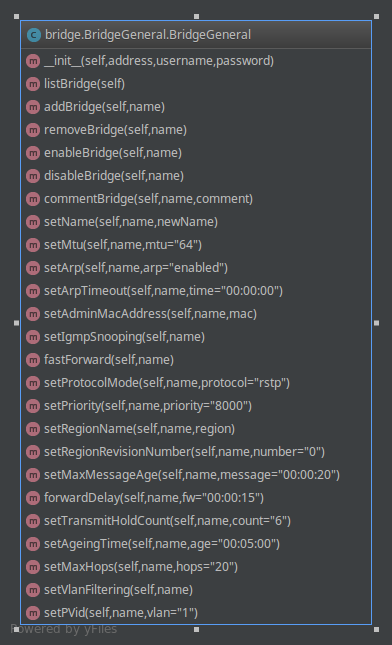
\includegraphics[scale=0.48]{../text/bridge.png}
\caption{UML diagram vybraného súboru bridgeArp}
\label{fig:bridge}
\end{figure}
\section{Zložka capsman}
\label{sec:capsmanchap}
Súčasťou zložky capsman sú súbory na centrálne nastevenie WiFi pomocou mikrotik funkcionality capsman. Capsman dovoľuje nastaviť a centrálne riadiť prístupové body na centrálnom smerovači.
Zložka pozostáva z:\begin{itemize}
\item Správu nakonfigurovaných položiek
\item Pridávanie, odstránenie, zapnutie, vypnutie a koment položiek
\item Modifikácia nakonfigurovaných položiek
\item Správa pripojených zariadení
\end{itemize}
\subsection{Popis tried zložky}
Zložka obsahuje:\begin{itemize}
\item \textbf{accessList} - trieda ošetruje nastavenie prístupých listov (access listov)
\item \textbf{accessListSet}- trieda ošetruje nastavenie už vytvorených access listov
\item \textbf{capAaa} - trieda ošetruje nastavenie autorizačného protokolu  AAA
\item \textbf{capManager} - trieda ošetruje nastavenie capsman managera
\item \textbf{capManagerInterfaces}- trieda ošetruje nastavenie capsman rozhraní
\item \textbf{capsmanRegTable} - trieda obsahuje zoznam zaregistrovaných zariadení  a ich publikácia (provisioning)
\item \textbf{channel} - trieda ošetruje nastavenie kanálov v rámci WIFi pre centrálne riadenie capsmanom
\item \textbf{channelSet} - trieda ošetruje nastavenie už existujúcich profilov kanálov 
\item \textbf{configChannels} - trieda ošetruje nastavenie kanálov v rámci globálnej konfigurácie WiFi v rámci  capsman
\item \textbf{configDatapath} - trieda očetruje nastavenie dátových ciest (datapath) v rámci globálneho konfiguračného súboru 
\item \textbf{configRates} - trieda ošetruje nastavenie povolených prenosových rýchlostí 
\item \textbf{configSecurity} - trieda ošetruje nastavenie bezpečnosti
\item \textbf{configurations} - trieda ošetruje management, pridávanie, odstránenie, povolenie, zakázanie a komentovanie konfiguračných súborov
\item \textbf{configWireless} - trieda ošetruje nastavenie Wireless rozhrania
\item \textbf{dataPath} - trieda ošetruje management dataPath, pridávanie, odstránenie, povolenie ,zakázanie a komentovanie
\item \textbf{dataPathSet} - trieda ošetruje nastavenie už existujúcich dátových ciest
\item \textbf{interface} - trieda ošetruje management rozhraní riadených capsmanom
\item \textbf{interfaceChannelSet} - trieda ošetruje nastavenie kanálov v rámci rozhrania
\item  \textbf{interfaceDatpathSet} - trieda ošetruje nastavenie dátových ciest v rámci konfigurácie rozhrania capsman
\item \textbf{interfaceRatesSet} - trieda ošetruje nastavenie povolených rýchlostí v rámci konfigurácie rozhrania capsmanom
\item  \textbf{interfaceSecuritySet} - trieda ošetruje nastavenie bezpečnosti v rámci capsman rozhrania
\item \textbf{interfaceSet} - trieda ošetruje základnú konfiguráciu rozhrania 
\item \textbf{interfaceWirelessSet} - trieda ošetruje nastavenie WiFi profilu
\item \textbf{provisioningSet} - trieda ošetruje možnosti publikácie konfigurácie - statické, dynamické
\item \textbf{provisioning} - trieda ošetruje management publikácie konfigurácií
\item \textbf{radio} -  trieda ošetruje nastavenie publikácie pripojných prístupových bodov
\item \textbf{rates} - trieda ošetruje management povolených prenosových rýchlostí
\item \textbf{ratesSet} - trieda ošetruje nastavenie prenosových rýchlostí
\item \textbf{remoteCap} - trieda ošetruje správu pripojených prístupových bodov - upgrade, publikáciu
\item \textbf{reselectChannnels} - trieda ošetruje výber druhého kanálu prístupového bodu
\item \textbf{secuirity} - trieda ošetruje management bezpečnostných profilov - pridávanie, odstránenie, povolenie ,zakázanie a komentovanie
\item \textbf{securitySet} - trieda ošetruje nastavenie bezpečnosti už existujúcich profilov
\end{itemize}
\subsection{Vybraný analyzovaný súbor}
Pre analýzu jedného súboru zo zložky je vybratý súbor \textit{configRates.py}. Jeho UML diagram je zobrazený na obrázku \ref{fig:capsman1} a zoznam jeho metód je popísaný v tabuľke \ref{tab:rates}.
\begin{figure}[H]
\centering
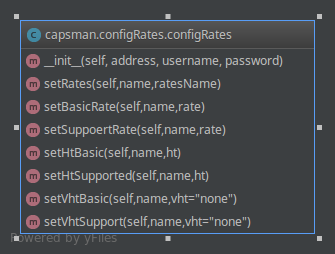
\includegraphics[scale=0.6]{../text/configRates.png}
\caption{UML diagram triedy configRates}
\label{fig:capsman1}
\end{figure}
\begin{table}[H]
\resizebox{\textwidth}{!}{%
\begin{tabular}{|c|c|c|c|}
\hline
Názov metódy & Vstup & Výstup & Vysvetlenie metódy \\ \hline
setRates & \begin{tabular}[c]{@{}c@{}}názov profilu,\\ nové meno\end{tabular} & slovník & Metóda premenuje profil \\ \hline
setBasicRate & \begin{tabular}[c]{@{}c@{}}názov profilu,\\ základné prenosové rýchlosti\end{tabular} & slovník & Metóda nastaví prenosovú rýchlosť. \\ \hline
setSuppoertRate & \begin{tabular}[c]{@{}c@{}}názov profilu,\\ podporované prenosové rýchlosti\end{tabular} & slovník & Metóda nastaví posporované prenosové rýchlosti. \\ \hline
setHtBasic & \begin{tabular}[c]{@{}c@{}}názov profilu,\\ základný prenosový kanál(y)\end{tabular} & slovník & Metóda nastaví prenosový kanál. \\ \hline
setHtSupported & \begin{tabular}[c]{@{}c@{}}názov profilu,\\ podporované prenosové kanály\end{tabular} & slovník & Metóda nastaví podporované prenosové kanály. \\ \hline
setVhtBasic & \begin{tabular}[c]{@{}c@{}}názov profilu,\\ základné virtuálne kanály\end{tabular} & slovník & Metóda nastaví prenosový virtuálny kanál. \\ \hline
setVhtSupport & \begin{tabular}[c]{@{}c@{}}názov profilu,\\ podporované prenosové virtuálne kanály\end{tabular} & slovník & Metóda nastaví podporované prenosové kanály. \\ \hline
\end{tabular}%
}
\caption{Popis triedy configRates}
\label{tab:rates}
\end{table}
\section{Zložka Dude}
Popisovaná zložka je obsah tried,ktoré nastavujú Dude monitorovací nástroj. Plnia rovnakú funkciu ako je to popísané v kapitolách \ref{sec:bridgechap} a \ref{sec:capsmanchap}. 
\subsection{Popis tried zložky}
Súčasťou zložky je nastavenie nástroja Dude na centrálny monitoring mikrotikov. Obsahuje súbory:\begin{itemize}
\item \textbf{Devices} - trieda ošetruje nastavenie monitorovaných zariadení
\item \textbf{Notifications} - trieda ošetruje nastavenie upozornení
\item \textbf{Probes} - trieda ošetruje nastavenie testovaní spojenia
\item \textbf{RosInfo} - trieda ošetruje výpis informácií ohľadom hardvéru a operačného systému routerOS
\item \textbf{Services} - trieda ošetruje nastavenie služieb
\item \textbf{Settings} - trieda ošetruje zapnutie a vypnutie Dude nástroju
\item \textbf{ostatné knižnice} - ostatné knižnice API nepodporuje
\end{itemize}
\subsection{Analýza vybraného súboru}
Vybraný analyzovaný súbor \textit{Devices.py} a jeho analýza je popísaná v rámci jeho UML diagramu na obrázku \ref{fig:dudedev} a zoznam metód je popísaný v tabuľke \ref{tab:devices}.
\begin{figure}[H]
\centering
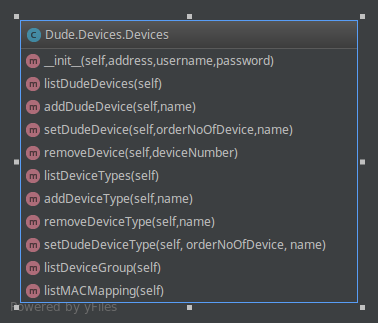
\includegraphics[scale=0.6]{../text/DudeDev.png}
\caption{UML diagram knižnice Devices}
\label{fig:dudedev}
\end{figure}
\begin{table}[H]
\resizebox{\textwidth}{!}{%
\begin{tabular}{cccc}
\hline
\multicolumn{1}{|c|}{Názov metódy} & \multicolumn{1}{c|}{Vstup} & \multicolumn{1}{c|}{Výstup} & \multicolumn{1}{c|}{Vysvetlenie metódy} \\ \hline
\multicolumn{1}{|c|}{listDudeDevices} & \multicolumn{1}{c|}{žiadny} & \multicolumn{1}{c|}{slovník} & \multicolumn{1}{c|}{Metóda vypíše zoznam Dude zariadení.} \\ \hline
\multicolumn{1}{|c|}{addDudeDevice} & \multicolumn{1}{c|}{názov zariadenia} & \multicolumn{1}{c|}{slovník} & \multicolumn{1}{c|}{Metóda pridá nové zariadenie} \\ \hline
\multicolumn{1}{|c|}{setDudeDevice} & \multicolumn{1}{c|}{\begin{tabular}[c]{@{}c@{}}číslo zariadenia,\\ meno zariadenia\end{tabular}} & \multicolumn{1}{c|}{slovník} & \multicolumn{1}{c|}{Metóda premenuje zariadenie.} \\ \hline
\multicolumn{1}{|c|}{removeDevice} & \multicolumn{1}{c|}{číslo zariadenia} & \multicolumn{1}{c|}{slovník} & \multicolumn{1}{c|}{Metóda zmaže zariadenie.} \\ \hline
\multicolumn{1}{|c|}{listDeviceTypes} & \multicolumn{1}{c|}{žiadny} & \multicolumn{1}{c|}{slovník} & \multicolumn{1}{c|}{Metóda zobrazí typy zariadení.} \\ \hline
\multicolumn{1}{|c|}{addDeviceType} & \multicolumn{1}{c|}{názov zariadenia} & \multicolumn{1}{c|}{slovník} & \multicolumn{1}{c|}{Metóda pridá nové zariadenie.} \\ \hline
\multicolumn{1}{|c|}{removeDeviceType} & \multicolumn{1}{c|}{názov profilu} & \multicolumn{1}{c|}{slovník} & \multicolumn{1}{c|}{Metóda zmaže typ zariadenia.} \\ \hline
\multicolumn{1}{l}{} & \multicolumn{1}{l}{} & \multicolumn{1}{l}{} & \multicolumn{1}{l}{} \\
\multicolumn{1}{l}{} & \multicolumn{1}{l}{} & \multicolumn{1}{l}{} & \multicolumn{1}{l}{} \\
\multicolumn{1}{l}{} & \multicolumn{1}{l}{} & \multicolumn{1}{l}{} & \multicolumn{1}{l}{}
\end{tabular}%
}
\caption{Tabuľka metód triedy Devices}
\label{tab:devices}
\end{table}
\section{Zložka Interfaces}
Popisovaná zložka je obsah tried,ktoré nastavujú rozhrania na mikrotiku. Medzi tieto rozhrania patria nastavenie VPN, ethernet, WiFi rozhraní a ďalších rozhraní. Plnia rovnakú funkciu ako je to popísané v kapitolách \ref{sec:bridgechap} a \ref{sec:capsmanchap} a ďalších kapitolách.
\subsection{Popis tried zložky}
Súčasťou zložky je nastavenie rohraní na mikrotiku. Patria sem triedy:
\begin{itemize}
\item \textbf{bonding} - trieda ošetruje nastavenie bonding rozhrania, rozhrania na nastevnie failover technológie súčasne s ďalšimi dvomi triedami na nastavenie bonding - \textbf{bondingGeneralSet} a \textbf{bondingSet} 
\item \textbf{detectInternet} - trieda detekuje internet na vybranom rozhraní
\item \textbf{eoipTunel} - trieda nastaví ethernet over IP rozhranie,spoločne s triedami \textbf{eoipSetGeneral} a \textbf{eoipSetLoopProtection}
\item \textbf{ethernet} - trieda nastaví ethernet rozhrania spoločne s triedami \textbf{ethernetSet}, \textbf{ethernetSetGeneral} a \textbf{ethernetLoopProtectionSet}
\item \textbf{greTunnel} - trieda nastaví rozhranie typu tunel GRE spoločne s triedou \textbf{greTunnelSet}
\item \textbf{interfaceList} - trieda nastaví listrozhraní spoločne s triedou \textbf{interfaceListSet}
\item \textbf{interfaces} - trieda zobrazí  a nastaví všetky rozhrania na mikrotiku
\item \textbf{interfaces} - trieda nastaví Long Term Evolution (LTE) rozhranie
\item \textbf{ipTunnel} - trieda nastaví IP tunel spoločne s triedou \textbf{ipTunnelSet}
\item \textbf{lists} - trieda nastaví listy rozhraní spoločne s triedou \textbf{listsSet}
\item \textbf{lteApn} - trieda nastaví prístupové LTE body spoločne s triedou \textbf{lteApnSet}
\item \textbf{vlan} - trieda nastaví VLAN spoločne s triedami \textbf{vlanLoopProtection} a \textbf{vlanSetGeneral}
\item \textbf{vrrp} - trieda nastaví zálohovací mechanizmus  Virtual Router Redoundency Protocol (VRRP) spoločne s triedami \textbf{vrrpGeneralSet, vrrpScriptSet a vrrpSetVrrp}
\end{itemize}
\subsection{Analýza vybraného súboru}
Vybraný súbor \textit{greTunnelSet.py} a jeho nastavenie je zobrazené v UML diagrame triedy na obrázku \ref{fig:gre} a popis tried je analyzovaný v tabuľke \ref{tab:greTunel}.
\begin{figure}[H]
\centering
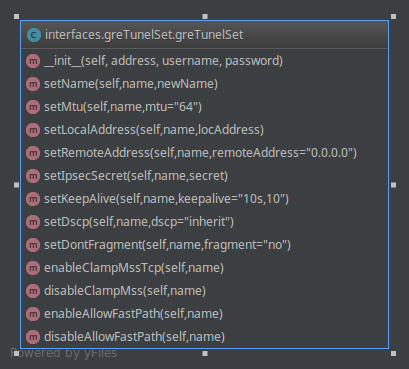
\includegraphics[scale=0.6]{../text/gre.png}
\caption{UML diagram greTunnelSet triedy}
\label{fig:gre}
\end{figure}
\begin{table}[H]
\resizebox{\textwidth}{!}{%
\begin{tabular}{|c|c|c|c|}
\hline
Názov metódy & Vstup & Výstup & Vysvetlenie metódy \\ \hline
setName & \begin{tabular}[c]{@{}c@{}}meno tunelu,\\ nové meno tunelu\end{tabular} & slovník & Metóda prmenuj tunel rozhranie. \\ \hline
setMtu & \begin{tabular}[c]{@{}c@{}}názov tunelu,\\ veľkoť MTU\end{tabular} & slovník & Metóda nastaví MTU rozhrania. \\ \hline
setLocalAddress & \begin{tabular}[c]{@{}c@{}}názov tunelu,\\ lokálna IP adresa\end{tabular} & slovník & Metóda nastaví lokálnu adresu. \\ \hline
setRemoteAddress & \begin{tabular}[c]{@{}c@{}}názov tunelu,\\ vzdialená  IP adresa\end{tabular} & slovník & Metóda nastaví vzdialenú IP adresu tunelu. \\ \hline
setIpsecSecret & \begin{tabular}[c]{@{}c@{}}názov tunelu,\\ heslo\end{tabular} & slovník & Metóda nastaví heslo na tunely. \\ \hline
setKeepAlive & \begin{tabular}[c]{@{}c@{}}názov tunelu,\\ keepalive interval\end{tabular} & slovník & Metóda nastaví keepalive interval. \\ \hline
setDscp & \begin{tabular}[c]{@{}c@{}}názov tunelu,\\ hodnota DSCP\end{tabular} & slovník & Metóda nastaví hodnotu DSCP. \\ \hline
setDontFragment & \begin{tabular}[c]{@{}c@{}}názov tunelu,\\ fragmentovanie\end{tabular} & slovník & Metóda nastaví možnosť fragmentovania (štandardne nie). \\ \hline
enableClampMssTcp & názov tunelu & slovník & Metóda zapne MSS pole pri fragmentovaní. \\ \hline
disableClampMss & názov tunelu & slovník & Metóda vypne MSS pole pri fragmentovaní. \\ \hline
enableAllowFastPath & názov tunelu & slovník & Metóda zapne funkciu tunelu "fast path". \\ \hline
disableAllowFastPath & názov tunelu & slovník & Metóda vypne funkciu tunelu "fast path". \\ \hline
\end{tabular}%
}
\caption{Tabuľka metód triedy greTunnelSet}
\label{tab:greTunel}
\end{table}
\newpage
\section{Zložka IPv4}
Popis  zložky IPv4 spočíva v nastavení rôznych IPv4 protokolov, bezpečnosti, prekladu adries,statického smerovania a ďalších možností. Triedy spočívajú globálnym popisom totožným k popisov v kapitolách \ref{sec:bridgechap}, \ref{sec:capsmanchap} a ďalších kapitolách.  
\subsection{Popis tried zložky}
Zložka obsahuje konguračné súbory nastavenie protokolov, adries, bezpečnosti a ďalších vecí na základe protokolu  IPv4. Zložka obsahuje:
\begin{itemize}
\item \textbf{Accounting} - Trieda ošetruje nastavenie zabezpečenia
\item \textbf{Addresses} - Trieda ošetruje nastavenie IP adries
\item \textbf{Arp} - Trieda ošetruje nastavenie Address Resolution Protocol (ARP) 
\item \textbf{DHCPClient} - trieda ošetruje nastavenie DHCP klienta
\item \textbf{DHCPRelay} - trieda ošetruje nastavenie DHCP relay agenta
\item \textbf{DHCPServer} - trieda ošetruje nastavenie DHCP serveru
\item \textbf{DNS} - triedy \textbf{DNScache, DNSGlobal a DNSstatic} ošetrujú nastavenie DNS protokolu global rieši management DNS serverov, cache rieši ošetrenie pridaných záznamov do DNS a static pridáva statické DNS záznamy
\item \textbf{Firewall} - triedy \textbf{Firewall-GeneralSetup, Action, Addresslist, AdvancedSetup,  Connections, ExtraSetup, Filter, L7Protocols,Mangle, NAT, ServicePorts}\\
\textbf{GeneralSetup} - trieda nastavuje základné vlastnosti firewallu
\textbf{Action} - trieda nastavuje akcie - povolenie, zakázanie, logovanie, ... \\
\textbf{AddressList} - trieda nastavuje address listy, skupiny adries v jednej premennej\\
\textbf{AdvancedSetup} - trieda ošetruje nastavenie pokročilých vlastností firewallu -napr. povolenie address listu, kde sa bude aplikovať, skupiny rozhraní, ...\\
\textbf{Conenctions} - trieda ošetruje správu spojení na mikrotiku
\textbf{ExstraSetup} - trieda ošetruje nastavenie napr. veľkosti hlavičky, sledovania počtu paketov za sekundu, ...\\
\textbf{Filter} - trieda ošetruje nastavenie a správu filter pravidiel\\
\textbf{L7Protocols} - trieda ošetruje nastavenie L7 protokolov - napr. torrent,...\\
\textbf{Mangle} - trieda ošetruje nastavenie Quality of Service (QoS)\\
\textbf{Network Address Translation (NAT)} - trieda ošetruje  nastavenie prekladu adries\\
\textbf{ServicePorts} - trieda ošetreuje servisné porty nastavené na firewalle
\item \textbf{Hotspot} - triedy H\textbf{otspotActive a HotspotCookies, Hotspothost, HotspotBridging, HotspotServer, HotspotServerProfile, HotspotServicePorts, HotspotUserProfile, HotspotUsers, HotspotWalledGarden, HotspotWalledGardenList} ošetrujú nastavenie WiFi hotspotu  a to konkrétne:\\
\textbf{HotspotActive} - trieda ošetruje nastavenie aktuálne bežiaceho hotspotu\\
\textbf{HotspotCookies} - trieda ošetruje nastavenie cookies\\
\textbf{Hotspothost} - - trieda ošetruje nastavenie správy hostov\\
\textbf{HotspotBridging} - trieda ošetruje nastavenie bridgu na hotspot\\
\textbf{HotspotServer} - trieda ošetruje nastavenie hotspot serveru\\
\textbf{HotspotServerProfile} - trieda ošetruje profil (konfiguračný) na nastavenie serveru hotspotu\\
\textbf{HotspotServicePorts} - trieda ošetruje správu servisných portov hotspotu\\
\textbf{HotspotUserProfile} - trieda ošetruje správu a nastavenie užívatšských profilov\\
\textbf{HotspotUsers} - trieda ošetruje správu pripojených užívateľov\\
\textbf{HotspotWalledGarden} - trieda ošetruje nastavenie bezpečnosti hotspotu\\
\textbf{HotspotWalledGardenList} - trieda ošetruje nastavenie "bezpečnostných listov"
\item \textbf{IPsec} - triedy \textbf{IPsecGroups, IPsecInstalledSA, IPsecKeys, IPsecModeCinfigs, IPsecPeers, IPsecPolicies, IPsecProposal, IPsecRemotePeers, IPsecUsers} nastavujú IPsec tunely a pozostávajú:\\
\textbf{IPsecGroups} - trieda ošetruje nastavenie IPsec skupín adries\\
\textbf{IPsecInstalledSA} - trieda spravuje nainštalované adresy\\
\textbf{IPsecKeys} - trieda ošetruje nastavenie kľúčov zabezpečenia\\
\textbf{IPsecModeCinfigs} - trieda ošetruje nastavenie módov\\
\textbf{IPsecPeers} - trieda ošetruje nastavenie fázy 1 IPsec\\
\textbf{IPsecPolicies} - trieda ošetruje nastavenie fázy 2 IPsec\\
\textbf{IPsecProposal} - trieda ošetruje nastavenie proposal profilov zabezpečenia tunelu\\
\textbf{IPsecRemotePeers} - trieda ošetruje správu vzdialených pripojených smerovačov do tunelu\\
\textbf{IPsecUsers} - trieda ošetruje správu užívateľov
\item \textbf{Neighbors} - triedy \textbf{NeighborDiscovery a Neighborlist} ošetrujú správu pripojených zariadení na mikrotik
\item \textbf{Packing} - trieda Packing ošetruje nastavenie a správu nainštalovaných balíčkov
\item \textbf{Pool} - triedy \textbf{Pool a PoolUsedAddresses} slúžia na konfiguráciu adresných rozsahov
\item \textbf{Route} - správa nastavení smerovania v triedach - \textbf{RouteVrf, RouteGeneral, RouteNexthops a RouteRules}\\
\textbf{RouteVrf} - správa nastavenia Vrf smerovania\\
\textbf{RouteGeneral} - správa hlavných smerovacích profilov\\
\textbf{RouteNexthops} - správa "next hop" adries\\
\textbf{RouteRules} - správa lokálnych smerovacích pravidiel
\item \textbf{Services} - trieda nastavuje povolené štandardné porty a služby na mikrotiku
\item \textbf{Settings} - trieda nastavuje globálne IPv4 nastavenie mikrotiku
\item \textbf{Samba} - triedy \textbf{Smb, SmbShare a smbUsers} ošetrujú nastavenie Samba protokolu\\
\textbf{Smb} - trieda globálne rieši nastavenie Samba profilov\\
\textbf{SmbShare} - trieda ošetruje nastavenie zdieľaných zložiek
\textbf{SmbUsers} - trieda ošetruje nastavenie Samba užívateľov
\item \textbf{Snmp} - trieda ošetruje nastavenie správu monitoringu zariadenia v triedach \textbf{Snmp, SnmpCommunity}\\
\textbf{Snmp} - trieda ošetruje globálne nastavenie SNMP protokolu\\
\textbf{SnmpCommunity} - trieda ošetruje globálne nastavenie komunnít(community stringov)
\item \textbf{Socks} - trieda ošetruje nastavenie socketov v triedach \textbf{Socks, SocksAccess a SocksConnections}
\item \textbf{Tftp} - trieda ošetruje nastavenie TFTP provozu
\item \textbf{TrafficFlow} - trieda ošetruje nastavenie kontroly trafiky v triedach \textbf{TrafficFlow a TrafficFlowIpFix}
\item \textbf{Upnp} - trieda ošetruje nastavuje UPNP v triedach \textbf{upnpinterface a upnpsettings} 
\item \textbf{Webproxy} - ošetrenie nastavenia Webového proxy serveru v súboroch:\\
\textbf{WebProxyAccess} - trieda ošetruje prístup k proxy serveru\\
\textbf{WebProxyCache} - trieda ošetruje správu cache pamäti proxy serveru\\
\textbf{WebProxyCacheContents} - trieda spravuje obsah pamäti\\
\textbf{WebProxyConenctions} - trieda spravuje pripojené zariadenia na proxy server\\
\textbf{WebProxyDirect} - trieda spravuje nastavenie priameho pripojenia na proxy server\\
\textbf{WebProxyLookup} - trieda ošetruje nastavenie lokálnej proxy DNS\\
\textbf{WebProxyRefreshes} - trieda ošetruje nastavenie obnovovacej frekvencie\\
\textbf{WebProxySettings} - trieda ošetruje globálne nastavenia proxy serveru
\end{itemize}
\subsection{Analýza vybraného súboru}
Vybraný súbor \textit{FirewallAddressist.py}popísaný UML diagramom na obrázku \ref{fig:addList} a obsah jeho metód je popísaný v tabuľke \ref{tab:addlist}.
\begin{table}[H]
\centering
\resizebox{\textwidth}{!}{%
\begin{tabular}{|c|c|c|c|}
\hline
Názov metódy & Vstup & Výstup & Vysvetlenie metódy \\ \hline
listAddressList & žiadny & slovník & Metóda vypíše zoznam address listov. \\ \hline
addAddressList & meno & slovník & Metóda pridá nový adress list. \\ \hline
removeList & meno & slovník & Metóda odstráni address list. \\ \hline
enableList & meno & slovník & Metóda zapne address list. \\ \hline
disableList & meno & slovník & Metóda vypne address list. \\ \hline
commentList & \begin{tabular}[c]{@{}c@{}}meno,\\ komentár\end{tabular} & slovník & Metóda nastaví komentár k záznamu v adress liste. \\ \hline
setName & \begin{tabular}[c]{@{}c@{}}číslo poradia záznamu,\\ meno\end{tabular} & slovník & Metóda zmení address list  v zázname. \\ \hline
setAddress & \begin{tabular}[c]{@{}c@{}}číslo poradia záznamu,\\ adresa\end{tabular} & slovník & Metóda zmení IP adresu položky. \\ \hline
setTimeout & \begin{tabular}[c]{@{}c@{}}číslo poradia záznamu,\\ timeout hodnota\end{tabular} & slovník & Metóda nastaví hodnotu timeoutu pre záznam v address liste. \\ \hline
\end{tabular}%
}
\caption{Obsah triedy FirewallAdressist}
\label{tab:addlist}
\end{table}
\begin{figure}[H]
\centering
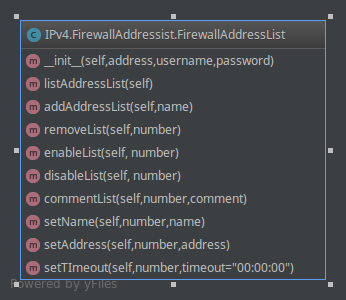
\includegraphics[scale=0.6]{../text/addList.png}
\caption{UML diagram triedy FirewallAddressist}
\label{fig:addList}
\end{figure}
\section{Zložka IPv6}
Podtstata zložky IPv6 je nastavenie IPv6 protokolu pozostavújecoho z DHCP pre IPv6, rozsahov adries, smerovania, firewallu a ďalších možností.
\subsection{Popis tried zložky}
Zložka obsahuje nastavenie funkcií prokolu IPv6 a zahrňuje:\begin{itemize}
\item \textbf{DHCPv6} - nastavenie protokolu DHCPv6 v triedach:\\
\textbf{DHCPRelay} - nastavenie DHCP Relay pre verziu IPv6\\
\textbf{DHCPServer} - nastavenie DHCP serveru\\
\textbf{DHCPv6Client} - nastavenie DHCPv6 klienta\\
\textbf{FirewallActions} - nastavenie firewall akcií - povolenie ,zahodenie, logovanie, ...\\
\textbf{FirewallAdvancedSetup} - nastavenie pokročilých vlastností firewallu napr. povolenie address listu, ...\\
\textbf{FirewallConnections} - Správa pripojení v o verzii IPv6\\
\textbf{FirewallExtraSetup} - Správa pokročilých nastavení napr. počet odoslaných paketov, ...\\
\textbf{FirewallFilter} -nastavenie filter pravidiel \\
\textbf{FirewallGeneralSetup} - nastavenie hlavných vlastností pravidlaa správa pravidiel\\
\textbf{FirewallMangle} - nastavenie QoS pre IPv6\\
\textbf{FirewallRaw} - nastavenie Raw (obdoba NAT)\\
\textbf{IPv6 AddressList}  - nastavenie address listu
\item \textbf{Addresses} - nastavenie a správa IPv6 adriesv triede \textbf{IPv6Addresses}
\item \textbf{Neighbors} - nastavenie a správa vyhľadávania pripojených zariadení v triede \textbf{IPv6NeighborDiscovery}
\item \textbf{Route} - správa smerovania v triede \textbf{IPv6Route}
\item \textbf{Settings} - správa nastavenia IPv6 na globálnej úrovni v triede \textbf{IPv6Settings}
\item \textbf{Neighbors} - správa pripojených zariadení v triede \textbf{Neighbors}
\item \textbf{Pool} - správa rozsahov adries v triede \textbf{Pool}
\end{itemize}
\subsection{Anylýza vybraného súboru}
Vybraný súbor \textit{FirewallManngle.py} je zobrazené UML diagramom triedy na obrázku \ref{fig:mangle} a obsah metód je zobrazený v tabuľke \ref{tab:ipv6mangle}.
\begin{table}[H]
\resizebox{\textwidth}{!}{%
\begin{tabular}{|c|c|c|c|}
\hline
Názov metódy & Vstup & Výstup & Vysvetlenie metódy \\ \hline
listRules & žiadny & slovník & Metóda vypíše zoznam pravidiel. \\ \hline
addRule & chain & slovník & Metóda pridá nové pravidlo. \\ \hline
removeRule & poradové číslo pravidla & slovník & Metóda odstráni pravidlo. \\ \hline
enableRule & poradové číslo pravidla & slovník & Metóda zapne pravidlo. \\ \hline
disableRule & poradové číslo pravidla & slovník & Metóda vypne pravidlo. \\ \hline
commentList & \begin{tabular}[c]{@{}c@{}}poradové číslo pravidla,\\ komentár\end{tabular} & slovník & Metóda nastaví komentár k pravidlu. \\ \hline
resetCounter & poradové číslo pravidla & slovník & Metóda zmaže počítadlo paketov a bytov pre konkrétne pravidlo. \\ \hline
resetAllCounters & žiadny & slovník & Metóda zmaže počítadlo všetkých pravidiel paketov a bytov. \\ \hline
\end{tabular}%
}
\caption{Tabuľka triedy FirewallMangle}
\label{tab:ipv6mangle}
\end{table}
\begin{figure}[H]
\centering
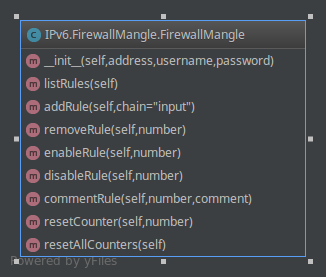
\includegraphics[scale=0.6]{../text/fwmangle.png}
\caption{UML diagram triedy FirewallMangle}
\label{fig:mangle}
\end{figure}
\section{Zložky KVM, log a makeSupportFile}
Obsahom zložiek je nastavenie virtuálneho mikrotiku, nastavenie logovania a vytvorenie súboru, ktorý je možné odslať na mikrotik podporu na analýzu. Celkový obsah je popísaný nižšie.
\subsection{Popis triedy zložky KVM}
Nastavenie virtuálnych mikrotikov alebo "mikrotiku v mikrotiku" je možné pomocou tzv. KVM. Zložka obsahuje triedy:\begin{itemize}
\item \textbf{KVM} - trieda na nastavenie virtualizácie na mikrotiku pomocou triedy \textbf{KVM}
\end{itemize}
Popis súboru \textit{KVM.py} je popísaný na obrázku \ref{fig:kvm}  a jeho obsah metód je popísaný v tabuľke \ref{tab:kvm}.
\begin{table}[H]
\resizebox{\textwidth}{!}{%
\begin{tabular}{|c|c|c|c|}
\hline
Názov metódy & Vstup & Výstup & Vysvetlenie metódy \\ \hline
listKVM & žiadny & slovník & Metóda zobrazí všetky virtuálne mikrotiky. \\ \hline
\end{tabular}%
}
\caption{Tabuľka metód triedy KVM}
\label{tab:kvm}
\end{table}
\begin{figure}[H]
\centering
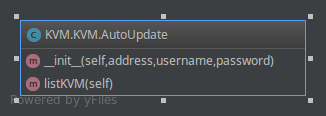
\includegraphics[scale=0.6]{../text/kvmfig.png}
\caption{UML diagram triedy KVM}
\label{fig:kvm}
\end{figure}
\subsection{Popis triedy zložky log}
Zložka log popisuje výpis systémového logu. Obsahuje triedy:\begin{itemize}
\item \textbf{log} - trieda log na výpis systémového logu
\end{itemize}
\begin{figure}[H]
\centering
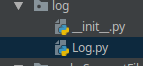
\includegraphics[scale=0.6]{../text/log.png}
\caption{Zoznam súborov zložky log}
\label{fig:log}
\end{figure}
Zoznam použitých metód je popísaný UML diagramom triedy na obrázku \ref{fig:logUML} a popísaný v tabuľke \ref{tab:log}.
\begin{table}[H]
\resizebox{\textwidth}{!}{%
\begin{tabular}{|c|c|c|c|}
\hline
Názov metódy & Vstup & Výstup & Vysvetlenie metódy \\ \hline
listLog & žiadny & slovník & Metóda zobrazí systémový log. \\ \hline
\end{tabular}%
}
\caption{Tabuľka metód triedy log}
\label{tab:log}
\end{table}
\begin{figure}[H]
\centering
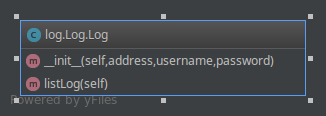
\includegraphics[scale=0.6]{../text/logUML.png}
\caption{UML diagram triedy log}
\label{fig:logUML}
\end{figure}
\subsection{Popis triedy makeSupportFile}
Zložka log obsahuje súbor makeSupportFile spoločne s triedou makeSupportFile, vytvorí a odošle súbor na podporu. Trieda makeSupport má na starosti vytvorenie súboru pre podporu na analýzu. Obsah súboru je popísaný v tabuľke \ref{tab:support} a UML diagramom triedy na obrázku \ref{fig:support}.
\begin{table}[]
\resizebox{\textwidth}{!}{%
\begin{tabular}{|c|c|c|c|}
\hline
Názov metódy & Vstup & Výstup & Vysvetlenie metódy \\ \hline
makeSupportFile & názov súboru & slovník & Metóda vytvorí súbor na podporu. \\ \hline
\end{tabular}%
}
\caption{Tabuľka metód triedy makeSupport}
\label{tab:support}
\end{table}
\begin{figure}[H]
\centering
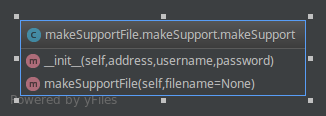
\includegraphics[scale=0.6]{../text/support.png}
\caption{UML diagram triedy makeSupport}
\label{fig:support}
\end{figure}
\section{Zložka Mesh}
Účelom zložky mesh je nastavenie tzv. mesh siete, mesh portov, správa pripojených zariadneí, atď. Zložka pozostáva obdobne ako je to v kapitolách \ref{tab:bridge1} a ďalších kapitolách.
\subsection{Popis tried zložky}
Zložka pozostáva z tried:
\begin{itemize}
\item \textbf{MeshFdb} - trieda ošetruje nastavenie a správu FDB prvkov
\item \textbf{MeshInterfaces} - trieda ošetruje nastavenie a správu mesh rozhraní
\item \textbf{MeshPorts} - trieda ošetruje nastaveniea správu mesh portov
\end{itemize}
\subsection{Analýza vybraného súboru}
Pre vybraný analyzovaný súbor \textit{MeshInterfaces.py}. Anaylýza tried je zobrazená na UML diagrame na obrázku \ref{fig:meshuml} a popis metód je popísaný v tabuľke \ref{tab:meshtab}.
\begin{table}[]
\resizebox{\textwidth}{!}{%
\begin{tabular}{|l|l|l|l|}
\hline
\multicolumn{1}{|c|}{Názov metódy} & \multicolumn{1}{c|}{Vstup} & \multicolumn{1}{c|}{Výstup} & \multicolumn{1}{c|}{Vysvetlenie metódy} \\ \hline
\multicolumn{1}{|c|}{listInterfaces} & \multicolumn{1}{c|}{žiadny} & \multicolumn{1}{c|}{slovník} & \multicolumn{1}{c|}{Metóda zobrazí všetky rozhrania.} \\ \hline
addInterface & meno rozhrania & slovník & Metóda pridá rozhranie. \\ \hline
removeInterface & meno rozhrania & slovník & Metóda zmaže rozhranie. \\ \hline
enableInterface & meno rozhrania & slovník & Metóda zapne rozhranie. \\ \hline
disableInterface & meno rozhrania & slovník & Metóda vypne rozhranie. \\ \hline
commentInterface & \begin{tabular}[c]{@{}l@{}}meno rozhrania,\\ komentár\end{tabular} & slovník & Metóda okomentuje rozhranie. \\ \hline
setName & \begin{tabular}[c]{@{}l@{}}meno rozhrania,\\ nové meno rozhrania\end{tabular} & slovník & Metóda premenuje rozhranie. \\ \hline
setMtu & \begin{tabular}[c]{@{}l@{}}meno rozhrania,\\ MTU\end{tabular} & slovník & Metóda nastaví beľkosť MTU. \\ \hline
setArp & \begin{tabular}[c]{@{}l@{}}meno rozhrania,\\ Arp mód (enabled štandardne)\end{tabular} & sloívník & Metóda nastaví mód ARP protokolu. \\ \hline
setArpTimeout & \begin{tabular}[c]{@{}l@{}}men orozhrania,\\ nastavenie hodnoty timeoutu\end{tabular} & slovník & Metóda nastaví timoeout ARP. \\ \hline
setAdminMac & \begin{tabular}[c]{@{}l@{}}meno rohrania,\\ admin MAC adresa\end{tabular} & slovník & Metóda nastaví admin adresu typu MAC. \\ \hline
setMeshPortal & meno rozhrania & slovník & Metóda nastaví mash portal. \\ \hline
setDefaultHopLimit & \begin{tabular}[c]{@{}l@{}}meno rozhrania,\\ limit (štandardne 2)\end{tabular} & slovník & Metóda nastaví maximálny počet "prekokov". \\ \hline
setPreqWaitingTime & \begin{tabular}[c]{@{}l@{}}meno rozhrania,\\ časová hodnota\end{tabular} & slovník & Metóda nastaví čas čakania záznamu v portále. \\ \hline
setPreqRetries & \begin{tabular}[c]{@{}l@{}}meno rozhrania,\\ počet opakovaní spojenia\end{tabular} & slovník & Metóda nastaví počet možných opakovaní spojenia. \\ \hline
setPreqDestinationOnly & meno rozhrania & slovník & Metóda nastaví spôsob spracovania dát v cieli. \\ \hline
setPreqReplyAndForward & meno rozhrania & slovník & Metóda nastaví spôsob spracovania odozvy prijatej správy. \\ \hline
setPrepLifetime & \begin{tabular}[c]{@{}l@{}}meno rozhrania,\\ doba života\end{tabular} & slovník & Metóda nastaví hodnotu doby života zariadenia na portály. \\ \hline
setRannInterval & \begin{tabular}[c]{@{}l@{}}meno rozhrania,\\ interval\end{tabular} & slovník & Metóda nastaví interval doby trvania metódy rann. \\ \hline
setRannPropagationDelay & \begin{tabular}[c]{@{}l@{}}meno rozhrania,\\ spozdenie\end{tabular} & slovník & Metóda nastaví delay systému rann. \\ \hline
setRannLifetime & \begin{tabular}[c]{@{}l@{}}meno rozhrania,\\ doba života\end{tabular} & slovník & Metóda nastaví dobu života rann. \\ \hline
reoptimizePaths & meno rozhrania & slovník & Metóda optimalizuje cestu k cieľu na rozhraní. \\ \hline
MeshTraceroute & \begin{tabular}[c]{@{}l@{}}rozhranie,\\ adresa,\\ limit (štandardne 255),\\ trvanie (štandardne 10 s)\end{tabular} & slovník & Metóda obsahuje traceroute na mash adresu. \\ \hline
\end{tabular}%
}
\caption{Tabuľka metód v triede MeshInterfaces}
\label{tab:meshtab}
\end{table}
\begin{figure}[H]
\centering
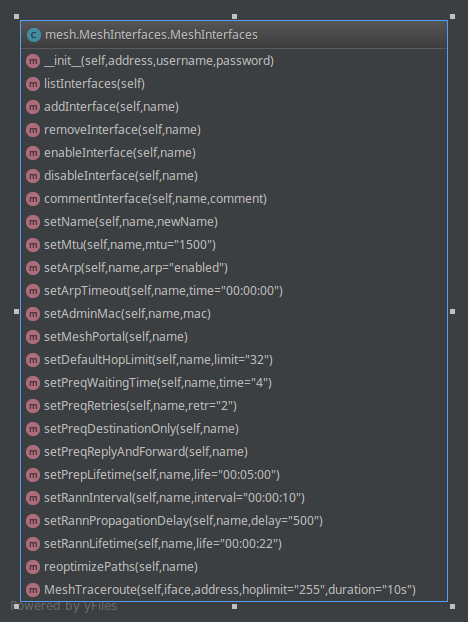
\includegraphics[scale=0.6]{../text/meshuml.png}
\caption{UML diagram triedy MeshInterfaces}
\label{fig:meshuml}
\end{figure}
\section{Zložka MPLS}
Multi Protocol Label Switing (MPLS) a jeho zložka globálne popísaná rovnakým spôsob ako zložka v kapitole \ref{tab:bridge1} a ďalších kapitolách. Triedy obsiahnuté v zložke slúžia na nastavenie MPLS prpeínania v počítačových sietiach.
\subsection{Popis tried zložky}
Zložka pozostáva z tried:
\begin{itemize}
\item \textbf{MplsAcceptFilter} - trieda ošetruje nastavenie  filktrovanie trafiky
\item \textbf{MplsAdvertiseFilter} - trieda ošetruje publikovanie filtrov
\item \textbf{MplsBgpVpls} - trieda ošetruje nastavenie VPLS v rámci  BGP protokolu
\item \textbf{MplsCiscoBgpVpls} - trieda ošetruje nastavenie VPLS v rámci technológií firmy CISCO
\item \textbf{MplsForwardingTable} - trieda ošetruje správu forwarding tabuľky
\item \textbf{MplsLdpInterface} - trieda ošetruje správu a nastavenie rozhraní MPLS
\item \textbf{MplsLdpNeighbor} - trieda ošetruje správu a nastavenie susedov
\item \textbf{MplsLocalBinding} - trieda ošetruje nastavenie  a správu lokálnych pripojení
\item \textbf{MplsRemoteBimndings} - trieda ošetruje nastavenie a správu vzdialených pripojení
\item \textbf{MplsSettings} - trieda ošetruje globálne nastavenie MPLS
\item \textbf{MplsVpls} - trieda ošeteruje správu a nastavenie VPLS
\item \textbf{TrafficEngInterface} - trieda ošetruje správu a nastavenie rozhrania prijímania trafiky
\item \textbf{TrafficEngPathState} - trieda ošetruje nastavenie a správu ciest tzv. "path state"
\item \textbf{TrafficResvState} - trieda ošeetruje nastavenie a správu tarfiky na strane príjímacej strany
\item \textbf{TrafficEngTraffInterface} - trieda ošetruje nastavenie a správu rozhraní riadenia trafiky
\item \textbf{TrafficEngTunnelPath} - trieda ošetruje nastavenie  a správu tunelov v rámci kontroly trafiky
\end{itemize}
\subsection{Anylýza vybraného súboru}
Vybraný analyzovaný súbor \textit{MplsLocalBinding.py} je popísaný jeho UML diagramom na obrázku \ref{fig:mplslocal} a v tabuľke \ref{tab:locbind}.
\begin{table}[H]
\centering
\resizebox{\textwidth}{!}{%
\begin{tabular}{|c|c|c|c|}
\hline
Názov metódy & Vstup & Výstup & Vysvetlenie metódy \\ \hline
listBindings & žiadny & slovník & Metóda zobrazí všetky preklady. \\ \hline
addBinding & žiadny & slovník & Metóda pridá preklad. \\ \hline
removeBinding & poradové číslo prekladu & slovník & Metóda zmaže záznam prekladu. \\ \hline
enableBinding & poradové číslo prekladu & slovník & Metóda zapne záznam prekladu. \\ \hline
disableBinding & ;poradové číslo prekladu & slovník & Metóda vypne záznam prekladu. \\ \hline
commentBinding & \begin{tabular}[c]{@{}c@{}}poradové číslo prekladu,\\ komentár\end{tabular} & slovník & Metóda okomentuje záznam prekladu. \\ \hline
setDstAddress & \begin{tabular}[c]{@{}c@{}}poradové číslo prekladu\\ cieľová IP adresa\end{tabular} & slovník & Metóda nastaví cieľovú adresu tunelu. \\ \hline
setLabel & \begin{tabular}[c]{@{}c@{}}poradové číslo prekladu,\\ označenie tunelu\end{tabular} & slovník & Metóda nastaví označenie tunelu. \\ \hline
\end{tabular}%
}
\caption{Tabuľka zoznamu metód triedy MplsLocalBindings}
\label{tab:locbind}
\end{table}
\begin{figure}[H]
\centering
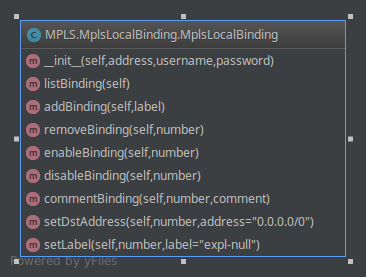
\includegraphics[scale=0.6]{../text/mplsuml.png}
\caption{UML diagram triedy MplsLocalBindings}
\label{fig:mplslocal}
\end{figure}
\section{Zložka PPP}
Úlohou zložky Point to point Protocol (PPP) je riadenie  a konfigurácia VPN spojenia rôznych typov napr. Open VPN (OVPN), SSTP, L2TP, ... Štruktúra zložky je rovnakaá ako v predchádzajúcich zložkách zahrňujúc kapitolu \ref{sec:bridgechap} a ďalšie kapitoly.
\subsection{Popis tried zložky}
Zložka obsahuje triedy:
\begin{itemize}
\item \textbf{activeConenctions} - trieda ošetruje  správu pripojených zariadení
\item \textbf{interfaceL2TP} - triedy\\
\textbf{interfaceL2TPClient} - nastavenie L2TP klienta\\
\textbf{interfaceL2TPSetGeneral} - nastavenie  globálnych nastavení klienta\\
\textbf{interfaceL2TPServer} - nastavenie L2TP servera\\
\textbf{interfaceL2TPServerBinding} - nastavenie spravovateľného L2TP server rozhrania\\
\textbf{interfaceL2TPSet} - globálne nastavenie rozhrania L2TP
\item \textbf{interfaceOvpn} - obsahuje triedy:\\
\textbf{interfaceOvpnClient} - nastavenie OVPN klienta\\
\textbf{interfaceOvpnClientSetDialOut} - nastavenie vytáčania OVPN klienta\\
\textbf{interfaceOvpnClientSetGenral} - globálne nastavenie OVPN klienta\\
\textbf{interfaceOvpnServer} - nastavenie a správa OVPN serverov\\
\textbf{interfaceOvpnServerBiding} - nastavenie spravovatľného rozhrania OVPN servera\\
\textbf{interfaceOvpnServerSet} - nastavenie OVPN servera
\item interfacePpp - obsahuje triedy:\\
\textbf{interfacePppClient} - nastavenie PPP klienta\\
\textbf{interfacePppClientSetGenral} - globálne nastavenie PPP klienta\\
\textbf{interfacePppClientSetPpp} - nastavenie PPP konfigurácie klienta\\
\textbf{interfacePppServerDialIn} - nastavenie vytáčania servera\\
\textbf{interfacePppServerSetGeneral} - nastavenie globálnej konfigurácie ppp server profilu\\
\textbf{pppAuthenticationAndAccounting} - nastavenie zabezpečenia PPP
\item interfacePppoe - obsahuje triedy:\\
\textbf{interfacePppoe} - správa rozhraní PPPoE\\
\textbf{interfacePppoeClient} - spráca PPPoE klientov\\
\textbf{interfacePppoeClientSetDialOut} - správa nastavenia vytášania klienta\\
\textbf{interfacePppoeSet} - nastavenie PPPoE rozhrania\\
\textbf{interfacePppoeSetGeneral} - nastavenie PPPoE globálneho nastavenia\\
\textbf{pppoe} - správa pppoe rozhraní\\
\textbf{pppoeSettings} - globálne nastavenie PPPoE
\item \textbf{interfacePptp} - obsahuje triedy:\\
\textbf{interfacePptpServer} - nastavenie Pptp servera\\
\textbf{interfacePptpServerBinding} - nastavenie spojení PPTP servera\\
\textbf{interfacePptpServerSetGenral} - hlavné nastavenie PPTP server profilu\\
\textbf{interfacePptpClientDialOut} - natsavenie vytáčania PPTP klienta\\
\textbf{interfacePptpClientSetGeneral} - základné  nastaveni PPTP klienta
\item \textbf{interfaceSstp} - obsahuje triedy:\\
\textbf{interfaceSstpClient} - nastavenie SSTP klienta\\
\textbf{interfaceSstpClientGeneralSet} - základné nastavenie SSTP klienta\\
\textbf{interfaceSstpClietSetDialOut} - nastavenie vytáčania SSTP klienta\\
\textbf{interfaceSstpServer} - nastavenie SSTP serveru\\
\textbf{interfaceSstpServerBinding} - nastavenie správy spojení servera SSTP\\
\textbf{interfaceSstpServerSet} - nastavenie SSTP servera
\item \textbf{l2tpSecrets} - nastavenie hesiel L2TP profilov
\item \textbf{profile} - obsahuje triedy:\\
\textbf{profileGeneral} - hlavné nastavenie užívateľov\\
\textbf{profileLimits} - natsavenie obmedzenia užívateľa\\
\textbf{profileProtocols} - nastavenie protokolov užívateľa\\
\textbf{profileQueue} - nastavenie fronty užívateľa\\
\textbf{profile} - správa užívateľov\\
\textbf{profileScripts} - nastavenie skriptov pri prihlásení a odhlásení užívateľa
\item \textbf{secrets} - trieda obsahuje:\\
\textbf{secrets} - správa hesiel\\
\textbf{secrtesSettings} - nastavenie hesiel
\end{itemize}
\subsection{Analyzovaný súbor}
Analyzovaný súbor \textit{interfacePppoeSetGeneral.py} je popísaný na UML diagrame \ref{fig:pppset} a v v tabuľke metód \ref{tab:ppptab}.
\begin{table}[H]
\centering
\resizebox{\textwidth}{!}{%
\begin{tabular}{|c|c|c|c|}
\hline
Názov metódy & Vstup & Výstup & Vysvetlenie metódy \\ \hline
setName & \begin{tabular}[c]{@{}c@{}}meno rozhrania,\\ nové meno rozhrania\end{tabular} & slovník & Metóda premenuje rozhranie. \\ \hline
setMaxMtu & \begin{tabular}[c]{@{}c@{}}men rozhrania,\\ nastavenie MTU\end{tabular} & slovník & Metóda nastaví veľkosť MTU. \\ \hline
setMaxMru & \begin{tabular}[c]{@{}c@{}}meno rozhrania,\\ veľkosťMRU\end{tabular} & slovník & Metóda nastaví veľkosť MRU. \\ \hline
setMrru & \begin{tabular}[c]{@{}c@{}}meno rozhrania,\\ veľkosťMRRU\end{tabular} & slovník & Metóda nastaví veľkosť MRRU. \\ \hline
setInterface & \begin{tabular}[c]{@{}c@{}}meno rozhrania,\\ rozhranie\end{tabular} & slovník & Metóda nastaví rozhranie na profil. \\ \hline
\end{tabular}%
}
\caption{Tabuľka popisu metód triedy interfacePppoeGeneralSet}
\label{tab:ppptab}
\end{table}
\begin{figure}[H]
\centering
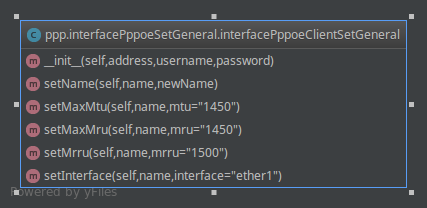
\includegraphics[scale=0.6]{../text/ppptab.png}
\caption{UML diagram triedy interfacePppoeGeneralSet}
\label{fig:pppset}
\end{figure}
\section{Zložka Queues}
Zložka popisuje nastavenie sieťovej fronty rôznych typov. Popis celkovej zložky je rovnaký ako v kapitole \ref{tab:bridge1} a ďalších kapitolách.
\subsection{Zoznam tried zložky}
Zložka obsahuje triedy:
\begin{itemize}
\item \textbf{QueueInterfaces} - nastavenie rozhraní
\item \textbf{QueueTree} - nastavenie stromu fronty
\item \textbf{QueueTypes} - nastavenie existujúcich a nových typov fronty
\item \textbf{SimpleQueues} - nastavenie jednoduchých front
\end{itemize}
\subsection{Analáza vybraného súboru}
Vybraný analyzovaný súbor \textit{QueueTree.py} je popísaný v tabuľke \ref{tab:tree} a na UML diagrame \ref{fig:queueTree}.
\begin{table}[H]
\centering
\resizebox{\textwidth}{!}{%
\begin{tabular}{|c|c|c|c|}
\hline
Názov metódy & Vstup & Výstup & Vysvetlenie metódy \\ \hline
listQueueTrees & žiadny & slovník & Metóda vypíše zoznam stromov. \\ \hline
addQueueTree & rodič & slovník & Metóda pridá nový strom. \\ \hline
removeQueueTree & menostromu & slovník & Metóda odtsráni strom. \\ \hline
disableQueueTree & meno stromu & slovník & Metóda vypne strom. \\ \hline
enableQueueTree & meno stromu & slovník & Metóda zapne strom. \\ \hline
commentQueueTree & \begin{tabular}[c]{@{}c@{}}meno stromu,\\ komentár\end{tabular} & slovník & Metóda okomentuje strom. \\ \hline
resetCounters & meno stromu & slovník & Metóda zmaže štatistiky stromu. \\ \hline
resetAllCounters & žiadny & slovník & Metóda zmaže všetky štatistiky. \\ \hline
setQueueName & \begin{tabular}[c]{@{}c@{}}meno,\\ nové meno\end{tabular} & slovník & Metóda premenuje strom. \\ \hline
setQueueParent & \begin{tabular}[c]{@{}c@{}}meno stromu,\\ rodič\end{tabular} & slovník & Metóda nastaví rodiča stromu. \\ \hline
setQueuePacketMark & \begin{tabular}[c]{@{}c@{}}meno stromu,\\ označenie paketu\end{tabular} & slovník & Metóda nastaví označenie paketov prichádzajúcich a odchádzajúcich zo stromu. \\ \hline
setQueueType & \begin{tabular}[c]{@{}c@{}}meno stromu,\\ typ fronty\end{tabular} & slovník & Metóda nastaví typ fronty. \\ \hline
setQueuePriority & \begin{tabular}[c]{@{}c@{}}meno stromu,\\ priorita\end{tabular} & slovník & Metóda nastaví prioritu fronty. \\ \hline
setQueueBuckezSize & \begin{tabular}[c]{@{}c@{}}meno stromu,\\ veľkosť úložiska fronty\end{tabular} & slovník & Metóda nastaví veľkosť úložiska na fronty. \\ \hline
setLimitAt & \begin{tabular}[c]{@{}c@{}}meno stromu,\\ limit\end{tabular} & slovník & Metóda nastaví monimálny limit na frontu. \\ \hline
setMaxLimit & \begin{tabular}[c]{@{}c@{}}meno stromu,\\ maximálny limit\end{tabular} & slovník & Metóda nastaví maximálny limit fronty. \\ \hline
setBurstTime & \begin{tabular}[c]{@{}c@{}}meno sstromu,\\ hodnota zhluku\end{tabular} & slovník & Metóda nastaví čas zhluku fronty. \\ \hline
setBurstThreshold & \begin{tabular}[c]{@{}c@{}}meno stromu,\\ prahová hranice\end{tabular} & slovník & Metóda nastaví prahovú hranicu zhluku front. \\ \hline
setBurstLimit & \begin{tabular}[c]{@{}c@{}}meno stromu,\\ limit zhluku\end{tabular} & slovník & Metóda nastaví limit zhluku. \\ \hline
\end{tabular}%
}
\caption{Tabuľka zoznamu metód triedy QueuTree}
\label{tab:tree}
\end{table}
\begin{figure}[H]
\centering
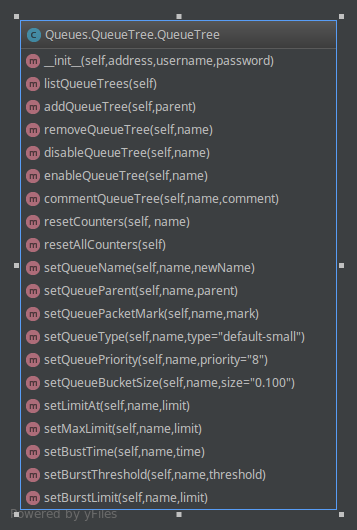
\includegraphics[scale=0.6]{../text/QueueTree.png}
\caption{UML diagram triedy QueueTree}
\label{fig:queueTree}
\end{figure}
\section{Zložka Radius}
Zložka Radius pozostáva z nastavenia Radiusu na mikrotiku. Radius pozostáva so súborov tried:\begin{itemize}
\item \textbf{Radius} - nastavenie a správa radiusu
\end{itemize}
V tabuľke \ref{tab:radius} a ma UML diagrame \ref{fig:radius} vidíme popis triedy Radius.
\begin{table}[H]
\centering
\resizebox{\textwidth}{!}{%
\begin{tabular}{|c|c|c|c|}
\hline
Názov metódy & Vstup & Výstup & Vysvetlenie metódy \\ \hline
listRadius & žiadny & slovník & Metóda vypíše zoznam RADIUS serverov. \\ \hline
addRadius & adresa & slovník & Metóda pridá nový RADIUS server. \\ \hline
removeRadius & poradové číslo serveru & slovník & Metóda odtsráni RADIUS server. \\ \hline
disableRadius & poradové číslo serveru & slovník & Metóda vypne RADIUS server. \\ \hline
enableRadius & poradové číslo serveru & slovník & Metóda zapne RADIUS server. \\ \hline
commentRadius & \begin{tabular}[c]{@{}c@{}}poradové číslo serveru,\\ komentár\end{tabular} & slovník & Metóda okomentuje RADIUS server. \\ \hline
printIncommingSettings & žiadny & slovník & Metóda vypíše štatistiky RADIUS serveru. \\ \hline
enableIncomming & žiadny & slovník & Metóda povolí prichádzajúcu trafiku. \\ \hline
setIncommingPort & port & slovník & Metóda nastaví port na prichádzajúcu trafiku. \\ \hline
disableIncommingTraffic & žaidny & slovník & Metóda vypne prichádzajúcu trafiku. \\ \hline
setQueuePacketMark & \begin{tabular}[c]{@{}c@{}}meno stromu,\\ označenie paketu\end{tabular} & slovník & Metóda nastaví označenie paketov prichádzajúcich a odchádzajúcich zo stromu. \\ \hline
resetIncommingCounters & žiadny & slovník & Metóda resetuje štatistiky spojenia. \\ \hline
resetAllRadiusCounters & žiadny & slovník & Metóda resetuje všetky štatistiky spojenia. \\ \hline
monitorRadius & \begin{tabular}[c]{@{}c@{}}poradové číslo serveru,\\ interval\end{tabular} & slovník & Metóda nastaví monitoring RADIUS serveru. \\ \hline
setRadiusService & \begin{tabular}[c]{@{}c@{}}poradové číslo serveru,\\ meno služby\end{tabular} & slovník & Metóda nastaví službu RADIUS. \\ \hline
setCalledId & \begin{tabular}[c]{@{}c@{}}poradové číslo serveru,\\ užívateľ\end{tabular} & slovník & Metóda nastaví vytáčaného užívateľa. \\ \hline
setDomain & \begin{tabular}[c]{@{}c@{}}poradové číslo serveru,\\ doména\end{tabular} & slovník & Metóda nastaví doménu. \\ \hline
setAddress & \begin{tabular}[c]{@{}c@{}}poradové číslo serveru,\\ adresa serveru\end{tabular} & slovník & Metóda nastaví adresu serveru. \\ \hline
setSecret & \begin{tabular}[c]{@{}c@{}}poradové číslo serveru,\\ heslo\end{tabular} & slovník & Metóda nastaví heslo na server. \\ \hline
setAuthenticationPort & \begin{tabular}[c]{@{}c@{}}poradové číslo serveru,\\ port\end{tabular} & slovník & Metóda nastaví autentikačný port. \\ \hline
setAccountingPort & \begin{tabular}[c]{@{}c@{}}poradové číslo serveru,\\ port\end{tabular} & slovník & Metóda nastaví port protokolu AAA. \\ \hline
setTimeout & \begin{tabular}[c]{@{}c@{}}poradové číslo serveru,\\ timeout\end{tabular} & slovník & Metóda nastaví timeout serveru. \\ \hline
enableAccountingBackup & poradové číslo serveru & slovník & Metóda zapne zálohovanie. \\ \hline
disableAccountingBackup & poradové číslo serveru & slovník & Metóda vypne zálohovanie. \\ \hline
setRealm & \begin{tabular}[c]{@{}c@{}}poradové číslo serveru,\\ doména\end{tabular} & slovník & Metóda nastaví sadu domén. \\ \hline
setSourceAddress & \begin{tabular}[c]{@{}c@{}}poradové číslo serveru,\\ zdrojová adresa\end{tabular} & slovník & Metóda nastaví zdrojovú adresu serveru. \\ \hline
\end{tabular}%
}
\caption{Tabuľka metód triedy Radius}
\label{tab:radius}
\end{table}
\begin{figure}[H]
\centering
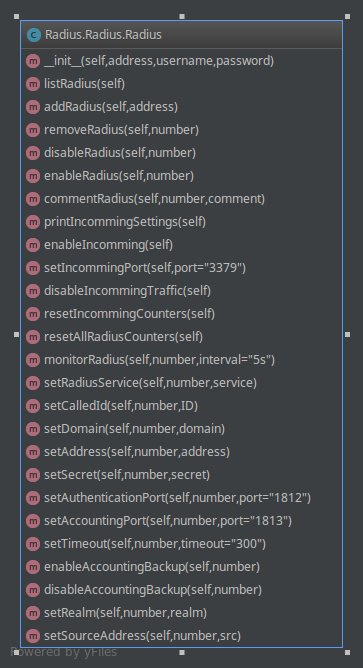
\includegraphics[scale=0.6]{../text/radiusPng.png}
\caption{UML diagram triedy Radius}
\label{fig:radius}
\end{figure}
\section{Zložka routing}
Zložka popisuje možnosti dynamického smerovania na mikrotiku. Rovnako ako kapitoly predtým, jej štruktúra je postavená na základe rovnakom ako je popísaný v kapitolách \ref{sec:bridgechap} a ostatných kapitolách.
\subsection{Zoznam tried zložiek}
Zložka pozostáva z tried:
\begin{itemize}
\item \textbf{BFD} - trieda ošetruje nastavenie BFD
\item \textbf{BGP} - triedy ošetrujú nastavenie BGP protokolu
\item \textbf{Filter} - triedy ošetrujú nastavenie BGP bezpečnosti
\item \textbf{IgmProxy} - triedy ošetrujú nastavenie IGMP proxy
\item \textbf{MME} - trieda ošetruje nastavenie MME
\item \textbf{OSPF} - triedy ošetrujú nastavenie OSPF
\item \textbf{PIM} - trieda ošetruje nastavenie PIM
\item \textbf{RIP} - trieda ošetruje nastavenie protokolu RIP
\item \textbf{RoutingFilter} - triedy ošetrujú nastavenie fiultrácie komunikácie protokolu BGP
\item \textbf{RP} - trieda ošetruje nastavenie Randevou point 
\item \textbf{VPNRoutes} - trieda ošetruje správu ciest VPN tunelu
\end{itemize}
\subsection{Analýza vybraného súboru}
Analýzou vybraného súboru \textit{RipNetworks.py} v UMl diagrame \ref{fig:rip}  a v tabuľke \ref{tab:rip}.
\begin{table}[H]
\centering
\resizebox{\textwidth}{!}{%
\begin{tabular}{|c|c|c|c|}
\hline
Názov metódy   & Vstup                                                                & Výstup  & Vysvetlenie metódy              \\ \hline
listNetwork    & žiadny                                                               & slovník & Metóda vypíše zoznam sietí.     \\ \hline
addNetwork     & sieť                                                                 & slovník & Metóda pridá novú sieť.         \\ \hline
removeNetwork  & poradové číslo siete                                                 & slovník & Metóda odtsráni sieť.           \\ \hline
disableNetwork & poradové číslosiete                                                  & slovník & Metóda vypne sieť.              \\ \hline
enableNetwork  & poradové číslo siete                                                 & slovník & Metóda zapne sieť.              \\ \hline
setNetwork     & \begin{tabular}[c]{@{}c@{}}poradové číslo siete,\\ sieť\end{tabular} & slovník & Metóda nastaví existujúcu sieť. \\ \hline
\end{tabular}%
}
\caption{Tabuľka popisu metód triedy RipNetworks}
\label{tab:rip}
\end{table}
\begin{figure}[H]
\centering
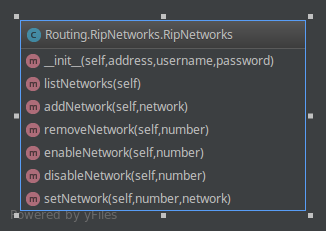
\includegraphics[scale=0.6]{../text/RipNetworks.png}
\caption{UML diagram súboru RipNetworks}
\label{fig:rip}
\end{figure}
\section{Zložka switch}
Cieľom zložkyswitch je nastavenie virtuálneho switchu na mikrotiku. Jeho infraštruktúra je identická s kapitolami \ref{sec:bridgechap} a ostatnými kapitolami. 
\subsection{Zoznam tried zložky}
Obsahom zložky sú triedy:
\begin{itemize}
\item \textbf{SwitchGeneral} -hlavné nastavenie prepínača
\item \textbf{SwitchHost} - nastavenie hostov
\item \textbf{SwitchPorts} -nastavenie portov prepínača
\item \textbf{SwitchRule} - nastavenie pravidiel filtrovania trafiky na prepínač
\item \textbf{SwitchVlan} - nastavenie virtuálnych LAN sietí
\end{itemize}
\subsection{Analýza vybraného súboru}
Analýza vybraného súboru \textit{switchPorts.py} jeodzrkadlená v UML diagrame \ref{fig:switchPort} a v tabuľke metód \ref{tab:switchPort}.
\begin{table}[H]
\centering
\resizebox{\textwidth}{!}{%
\begin{tabular}{|c|c|c|c|}
\hline
Názov metódy  & Vstup                                                                 & Výstup  & Vysvetlenie metódy                   \\ \hline
listPorts     & žiadny                                                                & slovník & Metóda vypíše zoznam portov switchu. \\ \hline
setVlanMode   & \begin{tabular}[c]{@{}c@{}}meno switchu,\\ vlan mód\end{tabular}      & slovník & Metóda nastaví VLAN mód portu.       \\ \hline
setVlanHeader & \begin{tabular}[c]{@{}c@{}}meno switchu,\\ hlavička VLAN\end{tabular} & slovník & Metóda nastaví hlavičku VLAN.        \\ \hline
setVlanId     & \begin{tabular}[c]{@{}c@{}}meno switchu,\\ VLAN ID\end{tabular}       & slovník & Metóda nastaví číslo VLAN.           \\ \hline
\end{tabular}%
}
\caption{Tabuľka zoznamu metód triedy switchPort}
\label{tab:switchPort}
\end{table}
\begin{figure}[H]
\centering
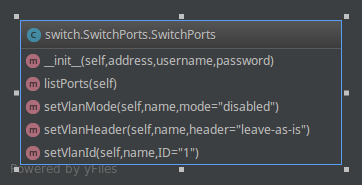
\includegraphics[scale=0.8]{../text/SwitchPorts.png}
\caption{UML digram triedy switchPorts}
\label{fig:switchPort}
\end{figure}
\section{Zložka System}
Účelom zložky system je nastavenie systémových nástrojov prvku mikrotik. Jej infraštruktúra je totožná k infraštruktúre kapitoly \ref{sec:bridgechap} a ďalších kapitol.
\subsection{Zoznam súborov zložky}
Zložka pozostáva zo súborov:
\begin{itemize}
\item \textbf{AutoUpdate} - správa automatických aktualizácií
\item \textbf{Certificates} - správa systémových certifikátov
\item \textbf{Console} - nastavenie konzolového portu
\item \textbf{Files} - správa súborvej infraštruktúry
\item \textbf{Health} - správa kontroly stavu hardvéru mikrotiku
\item \textbf{History} - správa histórie zmien na mikrotiku
\item \textbf{Identity} - správa nastavenia hostname
\item \textbf{Interfaces} -správa nastavenia konzolových rozhraní
\item \textbf{LCD} -správa nastavenia kontroly LCD displeja
\item \textbf{Licence} - správa licencie na mikrotiku
\item \textbf{Logging} -správa logovania 
\item \textbf{NTPClient} - správa klienta protokolu NTP
\item \textbf{NTPServer} - správa serveru protokolu NTP
\item \textbf{PackageManager} - správa aktualizácií mikrotiku a systémových balíkov
\item \textbf{ResetConfig} - správa resetovania konfigurácie mikrotiku
\item \textbf{RouterBoard} - správa získavania informácií o Routerboarde
\item \textbf{RouterOS} - správa informácií o operačnom systéme
\item \textbf{Scheduller} - správa plánovaných úloh
\item \textbf{Scripts} - správa systémových skriptov
\item \textbf{Services} - správa systémových služieb
\item \textbf{SpecialLogin} -správa šopeciálneho admin prihlasovacieho účtu
\item \textbf{SystemClock} - správa systémového času
\item \textbf{SystemMaintenance} - správa reštartu a vypnutia mikrotiku
\item \textbf{UPS} -správa konektoru na mikrotiku (AC adaptéru)
\item \textbf{user} -triedy nastavujú užívateľov, skupiny,...
\item \textbf{WatchDog} - sprva kontroly prvkov na mikrotiku
\end{itemize}
\subsection{Analýza vybraného súboru}
Vybraný analyzovaný súbor \textit{SystemMaintenance.py} je popísaný v UML diagrame \ref{fig:systemMaintenance} a v tabuľke \ref{tab:maintenance}.
\begin{table}[H]
\centering
\resizebox{\textwidth}{!}{%
\begin{tabular}{|c|c|c|c|}
\hline
Názov metódy   & Vstup  & Výstup  & Vysvetlenie metódy        \\ \hline
shutdownRouter & žiadny & slovník & Metóda vypne router       \\ \hline
rebootRouter   & žiadny & slovník & Metóda reštartuje router. \\ \hline
\end{tabular}%
}
\caption{Tabuľka metód triedy SystemMaintenance}
\label{tab:maintenance}
\end{table}
\begin{figure}[H]
\centering
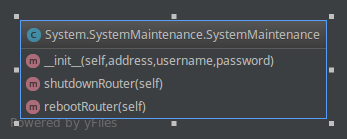
\includegraphics[scale=0.6]{../text/SystemMaintenance.png}
\caption{UML diagram triedy SystemMaintenance}
\label{fig:systemMaintenance}
\end{figure}
\section{Zložka tools}
Cieľom zložky tools je konfigurácia nástrojov prvku mikrotik. Jej infraštruktúra je identická infraštruktúre v zložke \ref{sec:capsmanchap} a ďalších kapitolách.
\subsection{Zoznam súborov zložky}
Zložka obsahuje:
\begin{itemize}
\item \textbf{BwServer} - trieda ošetruje nastavenieserveru správy šírky pásma
\item \textbf{BwTest} - trieda ošetruje testovanie šírky pásma
\item \textbf{Email} - trieda ošetruje odosielanie emailov z mikrotiku
\item \textbf{FloodPing} - trieda ošetruje tzv. "floodping" alebo "ping of death"
\item \textbf{Graphing} - trieda ošetruje nastavenie a export grafov
\item \textbf{IPscan} - trieda ošetruje skener IP adries
\item \textbf{MacServer} - trieda ošetruje nastavenie MAC serveru napr. na pripojenie pomoocu MAC adresy na winbox
\item \textbf{Netwatch} - trieda ošetruje nastavenie monitoringu trafiky na sieti
\item \textbf{PacketSniffer} - trieda ošetruje analyzátor paketov
\item \textbf{Ping} - trieda ošetruje štandardný nástroj overenia dostupnosti adresy ping
\item \textbf{PingSpeed} - trieda ošetruje meranie rýchlosti dostupnosti spojenia
\item \textbf{Profile} - trieda ošetruje nastavenie mikrotik profilu
\item \textbf{Romon} - trieda ošetruje nastavenie prístupu do romon módu (keď router nebootuje)
\item \textbf{SMS} - trieda ošetruje nastavenie odosielania správ na mobil z mikrotiku
\item \textbf{Telnet} - trieda ošetruje nastavenie pripojenia z mikrotiku pomocou protokolu telnet
\item \textbf{Torch} - trieda ošetruje zachytávanie trafiky
\item \textbf{Traceroute} - trieda ošetruje štandardný nástoj trasovania cesty traceroute
\item \textbf{TrafficGenerator} - trieda ošetruje nastavenie generátoru trafiky
\item \textbf{TrafficMonitorList} - trieda ošetruje správu trafiky
\end{itemize}
\subsection{Analýza vybraného súboru}
Analyzovaný vybraný súbor \textit{Netwatch.py} popísaný v tabuľke \ref{tab:tools} a na UML diagrame \ref{fig:netwatchuml}.
\begin{table}[H]
\centering
\resizebox{\textwidth}{!}{%
\begin{tabular}{|c|c|c|c|}
\hline
Názov metódy         & Vstup                                                                       & Výstup  & Vysvetlenie metódy                              \\ \hline
listNetwatchSessions & žiadny                                                                      & slovník & Metóda zobrazí spojenia netwatch.               \\ \hline
addNetwatch          & \begin{tabular}[c]{@{}c@{}}IP adresa,\\ interval,\\ timeout\end{tabular}    & slovník & Metóda pridá nový monitoring.                   \\ \hline
setNetwachHost       & \begin{tabular}[c]{@{}c@{}}číslo poradia spojenia,\\ IP adresa\end{tabular} & slovník & Metóda nastaví IP adresu existujúceho spojenia. \\ \hline
setNetwatchInterval  & \begin{tabular}[c]{@{}c@{}}číslo poradia spojenia,\\ interval\end{tabular}  & slovník & Metóda nastaví interval merania.                \\ \hline
setNetwatchTimeout   & \begin{tabular}[c]{@{}c@{}}číslo poradia spojenia,\\ interval\end{tabular}  & slovník & Metóda nastaví timeout spojenia.                \\ \hline
removeNetwatch       & poradové číslo spojenia                                                     & slovník & Metóda zmaže spojenie.                          \\ \hline
enableNetwatch       & poradové číslo spojenia                                                     & slovník & Metóda zapne spojenie.                          \\ \hline
disableNetwatch      & poradové číslo spojenia                                                     & slovník & Metóda vypne spojenie.                          \\ \hline
commentRule          & \begin{tabular}[c]{@{}c@{}}poradové číslo spojenia,\\ komentár\end{tabular} & slovník & Metóda okomentuje spojenie.                     \\ \hline
\end{tabular}%
}
\caption{Tabuľka metód súboru Netwatch}
\label{tab:tools}
\end{table}
\begin{figure}[H]
\centering
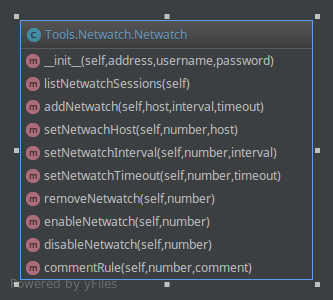
\includegraphics[scale=0.6]{../text/Netwatch.png}
\caption{UML diagram triedy Netwatch}
\label{fig:netwatchuml}
\end{figure}
\section{Zložka Wireless}
Zložka WIreless obsahuje nástroje na nastavenie WiFi spojenia. Jeho štruktúra je identická zložkám v kapitole \ref{sec:capsmanchap} a ďalších kapitolách.
\subsection{Zoznam tried zložky}
Zložka obsahuje triedy:
\begin{itemize}
\item \textbf{accessList} - triedy obsahujú nastavenie prístupových listov
\item \textbf{channels} - triedy obsahujú nastavenie prístupových kanálov WiFi
\item \textbf{connectionList} - trieda obsahuje správu pripojených zariadení
\item \textbf{interfaceCap} - triedy obsahujú nastavenie rozhraní Capsman
\item \textbf{interfaceNstremeDual} - triedy obsahujú nastavenie rozhraní NstremeDual
\item \textbf{interfaceRepeater} - trieda obsahuje nastavenie rozhrania Repeater
\item \textbf{interfaces} - trieda rieši správu všetkých rozhraní 
\item \textbf{interfaceSniffer} - trieda rieši pridanie tzv. "sniffera" na rozhranie
\item \textbf{interfaceVirtual} - triedy ošetrujú nastavenie virtuálnych rozhraní
\item \textbf{interfaceVirtualApBridge} - triedy ošetrujú nastavenie rozhrania AP Bridge
\item \textbf{interfaceVirtualBridge} - trieda ošetruje  nastavenie virtuálneho bridgu
\item \textbf{interfaceVirtualStationPseudoBridge} - trieda ošetruje nastavenie pseudobridgu
\item \textbf{interfaceVirtualStation} - trieda ošetruje nastavenie virtuálnej pracovnej stanice
\item \textbf{interfaceVirtualWds} - triedy ošetrujú nastavenie rohrania ako WDS
\item \textbf{interfaceWirelessAlignement} - trieda ošetruje zarovnanie pásma
\item \textbf{interfaceWpsClient} - trieda ošetruje nastavenie WPS klienta
\item \textbf{nstreme}- triedy ošetrujú nastavenie technológie nstreme dual
\item \textbf{registration} - trieda ošetruje správu zaregistrovaných zariadení
\item \textbf{security} - triedy ošetrujú nastavenie bezpečnosti WiFi siete napr. autentizácia cez RADIUS, šifrovanie,...
\item \textbf{wirelessSnooper} -nastavenie WiFi skenera 
\end{itemize} 
\subsection{Analýza vybraného súboru}
Analyzovaný súbor \textit{securityProfileRadius.py} je popísaný UML diagramom \ref{fig:wififig} a popis metód je v tabuľke \ref{tab:wifiradius}.
\begin{table}[H]
\centering
\resizebox{\textwidth}{!}{%
\begin{tabular}{|c|c|c|c|}
\hline
Názov metódy             & Vstup                                                                                   & Výstup  & Vysvetlenie metódy                                           \\ \hline
enableMacAuthentication  & meno profilu                                                                            & slovník & Metóda zapne autentizáciu na úrovni MAC adresy.              \\ \hline
disableMacAuthentication & meno profilu                                                                            & slovník & Metóda vypne autentizáciu na úrovni MAC adresy.              \\ \hline
enableMacAccounting      & meno profilu                                                                            & slovník & Metóda zapne započítavanie pripojenia na základe MAC adresy. \\ \hline
disableMacAccounting     & meno profilu                                                                            & slovník & Metóda vzpne započítavanie pripojenia na základe MAC adresy. \\ \hline
enableEapAccounting      & meno profilu                                                                            & slovník & Metóda zapne EAP (overenie doménovým menom).                 \\ \hline
disableEapAccounting     & meno profilu                                                                            & slovník & Metóda vypne EAP (overenie doménovým menom).                 \\ \hline
setInterimUpdate         & \begin{tabular}[c]{@{}c@{}}meno profilu,\\ update interval\end{tabular}                 & slovník & Metóda nastaví dobu aktualizácie.                            \\ \hline
setMacFormat             & \begin{tabular}[c]{@{}c@{}}meno profilu,\\ formát MAC adresy\end{tabular}               & slovník & Metóda nastaví formát MAC adresy.                            \\ \hline
setMacMode               & \begin{tabular}[c]{@{}c@{}}meno profilu,\\ mód autentizácie na základe MAC\end{tabular} & slovník & Metóda naství mód MAC adries.                                \\ \hline
setMacCahingTime         & meno profilu                                                                            & slovník & Metóda nastaví dobu cashovania záznamov.                     \\ \hline
\end{tabular}%
}
\caption{Tabuľka metód triedy securityProfileRadius}
\label{tab:wifiradius}
\end{table}
\begin{figure}[H]
\centering
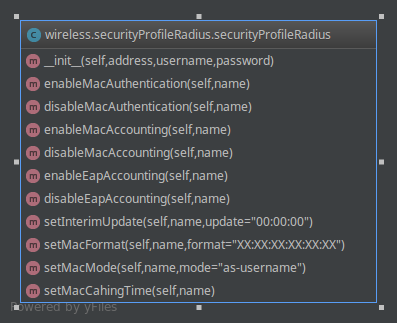
\includegraphics[scale=0.6]{../text/securityProfileRadius.png}
\caption{UML diagram triedy securityProfileRadius}
\label{fig:wififig}
\end{figure}